%!TEX root = /Users/jakubkonka/Thesis/Thesis.tex
\chapter{Network Selection Mechanism in the Digital Marketplace} % (fold)
\label{cha:network_selection_mechanism_in_the_digital_marketplace}

\minitoc
\vspace{10mm}

The world of mobile and wireless communications is becoming increasingly diverse in terms of different wireless access technologies available: in addition to the already established family of technologies (GSM, 3G, and WiFi), the cutting-edge 4G technology, LTE, is gradually being rolled out in many countries including the USA \cite{VerizonLTEUSA}, or is actively being tested for the eventual implementation in the near future in countries such as the UK \cite{BBCLTEUK}. In an environment of such diversity and heterogeneity, where each wireless access technology has its own distinct characteristics, network selection mechanisms provide a more resource efficient way of handling communications services by matching the services' required quality with the characteristics of a particular access technology \cite{HossainBeaubrun09, HossainTalebiFard09}. The importance of such mechanisms is further emphasized by the fact that multimode devices such as smartphones (iPhones, Android phones, BlackBerry phones) and tablets (iPads, Android tablets) currently dominate the market enabling users to connect to many of the available wireless access technologies, including WiFi and 3G.

This diversity combined with the availability of smartphones opens exciting, new possibilities in both the technological and economic sense. The exclusive one-to-one mapping between network operators and subscribers need no longer hold; when requesting a service (e.g., phone call, web browsing, email), the network selection mechanism will be responsible for selecting the network operator and the access technology that best matches the quality requirements of the service. From the subscribers' perspective, this will lead to the ability to seamlessly connect at any time, at any place, and to the technology offering the most optimal quality available for the best price: a paradigm referred to as \emph{Always Best Connected} \cite{ABC03}. From the network operators' perspective, the integration of wireless access technologies will allow for more efficient usage of network resources, and might be the most economic way of providing both universal coverage, and broadband access \cite{HossainBeaubrun09}.

However, there also exists the possibility of a `tussle' since there are many different actors with opposing interests involved \cite{Clark02}. For example, it is in the best interest of subscribers to obtain the highest quality of the service for the lowest price. Network operators, on the other hand, aim to maximize their profit by performing efficient load balancing. Furthermore, the situation may become even more complex should the service provision be separated from the network operators; that is, if the service provision is handled by a separate entity, service provider, while network operators are left with handling of the transport provision \cite{DMBushTussle09}. Therefore, the problem of network selection, which was considered to be technologically difficult, can also be considered to be the problem of economics where communications services, traded on a per service basis, are the electronic goods that are sold to the subscribers.

In this research, we analyze the network selection mechanism proposed in the Digital Marketplace---a market-based framework where network operators compete in a procurement auction-based setting for the right to transport the subscriber's requested service over their infrastructure \cite{DMLeBodic00}. Within this framework, the network selection mechanism is akin to a market selling mechanism where network operators assume the role of the sellers/bidders\footnote{Henceforth, sellers and bidders are used interchangeably unless stated otherwise.} and subscribers are the buyers of the transport services offered by the network operators. In this way, the Digital Marketplace strives to address the tussle between the actors involved, and thus, attempts to address both technological as well as economic constraints of the problem.

We create a simple economic model of the auction, and characterize the equilibrium under generic assumptions about the costs distributions of the network operators. Furthermore, the equilibrium is explicitly derived under more specific assumptions about the model; that is, two network operators and costs drawn from uniform distributions. In this case, we also analyze how the buyer can influence the bidding process in order to choose the network operator who matches their preferences about the service; for example, trading off quality for a lower price.

The rest of this chapter is organized as follows.

\section{Related Literature} % (fold)
\label{sec:related_literature}
Over the last decade, several papers have explored the problem of intelligent network selection in heterogeneous wireless access networks. Antoniou et al., and Charlias et al.~model the problem as a noncooperative game between wireless access networks with the aim of obtaining the best possible trade-off between the efficiency and the available capacity of networks, while, at the same time, satisfying the requested quality by the subscribers \cite{Antoniou07, Charilas08}. Ormond et al.~propose an algorithm for cost-oriented and performance-aware network selection that maximizes consumer surplus \cite{OrmondCS106, OrmondCS206}. Niyato et al.~propose two algorithms based on evolutionary game theory for a network selection mechanism which performs intelligent load balancing so that network congestion and performance degradation can be avoided \cite{Niyato09}. Additionally, the same authors model the user churning behavior in heterogeneous wireless access networks using evolutionary game theory \cite{NiyatoHossainConf2008}. Khan et al.~model the problem as a procurement second-price sealed-bid auction where network operators bid for the right to service the subscriber's request \cite{Khan110, Khan210}. Zhu et al.~build upon the work reported in~\cite{Niyato09}, and explore the dynamics of network selection, using Bayesian evolutionary game theory, in an environment where subscribers have only limited (incomplete) information about each others preferences \cite{ZhuNiyato2010}. Finally, Irvine et al.~propose a market-based framework called the Digital Marketplace where network operators compete in a variant of a procurement first-price sealed-bid auction for the right to transport the subscriber's requested service over their infrastructure \cite{DMLeBodic00, DMIrvine01, DMIrvine02}.
% section related_literature (end)

\section{The Digital Marketplace} % (fold)
\label{sec:the_digital_marketplace}
The Digital Marketplace (DMP) is a market-based framework for trading wireless communications services. In its simplest form, there are four main groups of actors involved in the operation of the DMP: \emph{subscribers}, \emph{service providers}, \emph{network operators}, and \emph{market provider}. The subscribers are the end-users of the communications services. Furthermore, they can interact with the network operators either directly or through the service provider. In the former case, they act as the buyer in the DMP, and directly negotiate with the interested network operators. In the latter case, on the other hand, the service provider acts as an intermediary between the subscribers and the network operators, and hence, acts as the buyer during the negotiation process. Lastly, the market provider is tasked with operating the DMP; thus providing common platform for all actors involved. It is left open-ended who should be the market provider; however, one of the following three choices is the most likely: a regulatory body, a consortium of network operators, or a single network operator on behalf of the regulatory body \cite{DMIrvine02}.

The process of negotiation (or the network selection mechanism) in the DMP is based on a procurement first-price sealed-bid auction where the network operators represent the sellers/sellers, and the subscriber or the service provider is the buyer. Unlike in a standard procurement first-price sealed-bid auction, the winning bid is a weighted (convex) combination of both the network operator's monetary bid and their reputation rating; we will refer to it as the \emph{compound bid}. The network operator is elected as the winner of the auction if their compound bid is the lowest in value, and accrues their monetary bid minus the cost of transporting the service. The monetary bid is equivalent to the price of transporting the service by the network operator. The precise definition of the price is left open-ended; one possibility, for example, would be to charge the buyer per unit of bandwidth. The weights in the compound bid are set by the buyer before each auction, and are announced to the network operators. This effectively gives the buyer the freedom to choose any combination ranging from: a low price for the service but also poor quality; to a high quality but for a high price \cite{DMLeBodic00}.

Since the communications services are traded on an individual service level, it might be difficult for the buyer to judge the overall quality of the services supplied by a particular network operator \cite{DMIrvine02}. Therefore, the DMP maintains a reputation rating for each network operator. The reputation rating is directly proportional to the number of services that have prematurely been decommitted in the past by the respective network operator; i.e., the lower the number of the decommitted service requests, the lower the reputation rating \cite{DMLeBodic00}. The reputation of the respective network operator, on the other hand, is inversely proportional to the reputation rating; i.e., the lower the rating, the higher the reputation.

Although the DMP was developed when GSM was widespread and 3G was in its infancy, it can still be adapted to the current scenario where we witness the domination of packet-switched data communications over the traditional circuit-switched cellular telephony \cite{Ericsson2011}.
% section the_digital_marketplace (end)

\section{Notation and Preliminaries} % (fold)
\label{sec:notation_and_preliminaries}
The following notation and concepts are assumed throughout the rest of this chapter.

\subsection{Set Theory} % (fold)
\label{sub:notation_set_theory}
Let $A$ be a set defined using the following notation $A = \{x: \mathcal{P}x\}$. This notation is referred to as \emph{set-builder notation} and, in this particular example, the unique set $A$ consists of all $x$ such that the condition $\mathcal{P}x$ is satisfied \cite{Carter2001}. A more concrete example: $B = \{x\in\mathbb{R}: x\ge 0\}$. Here, $B$ is the subset of the real line consisting of all non-negative real numbers; i.e., $B=\mathbb{R}_+$.

Let $f: X\to Y$ be a one-to-one and onto function. Then we call $f$ invertible and denote the inverse of $f$ as $f^{-1}$ with the property that for all $x\in X$ and $y\in Y$, $f(x) = y$ and $f^{-1}(y) = x$.
% subsection set_theory (end)

\subsection{Probability Theory and Statistics} % (fold)
\label{sub:notation_probability}
Let $X$ denote a continuous random variable (r.v.) with the support $[a, b]$, where $a < b$ and $a, b \in\nobreak\mathbb{R}$. By $F_{X}$ we mean a cumulative distribution function of the $X$ r.v.; therefore, for any $x\in\mathbb{R}$, $F_{X}(x) = P\{X \le x\}$, where $P\{X\le x\}$ denotes the probability of the event such that $X\le x$. If $F_{X}$ admits a density function, it shall be denoted by $f_{X} \equiv \frac{d}{dx}F_{X}$. If it is clear from the context which variable is considered random, we shall drop the subscript; that is, $F_{X}\equiv F$.

The expected value of $X$, denoted by $E[X]$, is defined as $E[X] = \int_{-\infty}^{\infty} xdF(x)$. Similarly, if $u$ is a function of $X$, then the expected value of $u(X)$ is defined as $E[u(X)] = \int_{-\infty}^{\infty} u(x)dF(x)$.

Let $X_1, \ldots, X_n$ be independent continuous r.v.s with distribution function $F$ and density function $f\equiv \frac{d}{dx}F$. If we let $X_{i:n}$ denote the $i$th smallest of these r.v.s, then $X_{1:n}, \ldots,X_{n:n}$ are called the \emph{order statistics} \cite{Arnold08,David03}. In the event that the r.v.s are independently and identically distributed (i.i.d.), the distribution of $X_{i:n}$ is
\begin{equation}
	\label{eq:iid_cdf}
	F_{X_{i:n}}(x) = \sum_{k=i}^{n} \binom{n}{k} (F(x))^k (1-F(x))^{n-k},
\end{equation}
while the density of $X_{i:n}$ can be obtained by differentiating Equation~\eqref{eq:iid_cdf} with respect to $x$ \cite{Ross10}. Hence,
\begin{equation}
	\label{eq:iid_pdf}
	f_{X_{i:n}}(x) = \frac{n!}{(n-i)!(i-1)!} f(x) (F(x))^{i-1} (1-F(x))^{n-i}.
\end{equation}

Let $X_1,\ldots,X_n$ be i.i.d.~r.v.s with finite mean $\mu$. Let
\begin{equation*}
  \bar{X}(n) = \frac{\sum_{i=1}^n X_i}{n}.
\end{equation*}
Then, for sufficiently large $n$, $\bar{X}(n)$ provides a reasonable approximation of $\mu$ \cite{LawChapter42007}. This result is known as the Strong Law of Large Numbers,
\begin{thm}[Strong Law of Large Numbers]
$\bar{X}(n)\rightarrow\mu$ with probability $1$ as $n\rightarrow\infty$.
\end{thm}
The proof of this theorem can be found in Chung's ``A Course in Probability Theory'' \cite{Chung2001}.
% subsection notation_probability (end)

\subsection{Optimization Theory} % (fold)
\label{sub:notation_optimisation_theory}
The following theorem on nonlinear constrained optimization will also be used in this chapter.
\begin{thm}[Karush-Kuhn-Tucker Conditions]
Let $f:\mathbb{R}^n\to\mathbb{R}$ be a concave function, $g_i:\mathbb{R}^n\to\mathbb{R}$ be convex functions for $i=1,\ldots,m$, and $h_j:\mathbb{R}^n\to\mathbb{R}$ be affine functions for $j=1,\ldots,l$. Then $\mathbf{x}^*\in\mathbb{R}^n$ is an optimal point for the following optimization problem:
\begin{equation*}
	\left\{
	\begin{array}{rl}
		\max &f(x_1,\ldots,x_n)\\
		\text{subject to} &g_1(x_1,\ldots,x_n)\le 0\\
		& \vdots\\
		&g_m(x_1,\ldots,x_n)\le 0\\
		&h_1(x_1,\ldots,x_n) = 0\\
		& \vdots\\
		&h_l(x_1,\ldots,x_n) = 0
	\end{array}
	\right.
\end{equation*}
if and only if there exist unique multipliers $\bm{\lambda}=(\lambda_1,\ldots,\lambda_m)\ge 0$ and $\bm{\mu}=(\mu_1,\ldots,\mu_l)\in\mathbb{R}$ such that the Lagrangian
\begin{equation*}
	L(\mathbf{x},\bm{\lambda},\bm{\mu}) = f(\mathbf{x}) - \sum_{i=1}^m\lambda_i g_i(\mathbf{x}) - \sum_{j=1}^l\mu_j h_j(\mathbf{x})
\end{equation*}
is stationary at $(\mathbf{x}^*,\bm{\lambda},\bm{\mu})$, that is,
\begin{equation*}
	\nabla L(\mathbf{x}^*,\bm{\lambda},\bm{\mu}) = \nabla f(\mathbf{x}^*) - \sum_{i=1}^m\lambda_i \nabla g_i(\mathbf{x}^*) - \sum_{j=1}^l\mu_j \nabla h_j(\mathbf{x}^*) = \mathbf{0},
\end{equation*}
and satisfies the complementary slackness conditions
\begin{equation*}
	\lambda_i g_i(\mathbf{x}^*)=0 \quad\text{for } i=1,\ldots,m.
\end{equation*}
\end{thm}
\noindent The proof of this theorem can be found in any literature discussing mathematical optimization theory such as Carter's ``Foundations of Mathematical Economics'' \cite{Carter2001}.
% subsection notation_optimisation_theory (end)

\subsection{Theory of Games with Incomplete Information} % (fold)
\label{sub:notation_theory_of_games_with_incomplete_information}
Let $\Gamma^B = [N, \{S_i\}, \{u_i\},\Theta,F]$ be a \emph{Bayesian game with incomplete information}. Formally, in this type of games, each player $i\in N$ has a utility function $u_i(s_i, s_{-i}, \theta_i)$, where $s_i\in S_i$ denotes player $i$'s action, $s_{-i}\in S_{-i} = \vartimes_{j\neq i}S_j$ denotes actions of all other players different from $i$, and $\theta_i\in\Theta_i$ represents the type of player $i$. Letting $\Theta = \vartimes_{i\in N} \Theta_i$, the joint probability distribution of the $\theta\in\Theta$ is given by $F(\theta)$, which is assumed to be common knowledge among the players\footnote{For more in-depth treatment of the theory of games see for example \cite{Myerson97, Gibbons92, MicroTheory}.}.

In game $\Gamma^B$, a \emph{pure strategy} for player $i$ is a function $\psi_i: \Theta_i\to S_i$, where for each type $\theta_i\in \Theta_i$, $\psi_i(\theta_i)$ specifies the action from the feasible set $S_i$ that type $\theta_i$ would choose. Therefore, player $i$'s pure strategy set $\Psi_i$ is the set of all such functions.

Player $i$'s \emph{expected utility} given a profile of pure strategies $(\psi_1,\ldots,\psi_{|N|})$ is given by
\begin{equation}
	\label{eq:def_exp_utility}
	\tilde{u}_i(\psi_1,\ldots,\psi_{|N|}) = E[u_i(\psi_1(\theta_1),\ldots,\psi_{|N|}(\theta_{|N|}),\theta_i)],
\end{equation}
where the expectation is taken over the realizations of the players' types, $\theta\in\Theta$. Now, in game $\Gamma^B$, a strategy profile $(\psi_1^*,\ldots,\psi_{|N|}^*)$ is a \emph{pure-strategy Bayesian Nash equilibrium} if it constitutes a Nash equilibrium of game $\Gamma^N = [N, \{\Psi_i\},\{\tilde{u}_i\}]$; that is, if for each player $i\in N$,
\begin{equation}
	\label{eq:def_bayesian_nash_eq}
	\tilde{u}_i(\psi^*_i,\psi^*_{-i}) \ge \tilde{u}_i(\psi_i,\psi^*_{-i})
\end{equation}
for all $\psi_i\in\Psi_i$, where $\tilde{u}_i(\psi_i,\psi_{-i})$ is defined as in Equation~\eqref{eq:def_exp_utility}.

Alternatively, a strategy profile $(\psi_1^*,\ldots,\psi_{|N|}^*)$ constitutes a pure-strategy Bayesian Nash equilibrium in game $\Gamma^B$ if and only if, for all $i\in N$ and all $\hat{\theta}_i\in\Theta_i$ occurring with positive probability
\begin{equation}
	\label{eq:prop_bayesian_nash_eq}
	E[u_i(\psi^*_i(\hat{\theta}_i),\psi^*_{-i}(\theta_{-i}),\hat{\theta}_i)\mid\hat{\theta}_i] \ge
	E[u_i(s'_i,\psi^*_{-i}(\theta_{-i}),\hat{\theta}_i)\mid\hat{\theta}_i]
\end{equation}
for all $s'_i\in S_i$, where the expectation is taken over realizations of the other players' types, $\theta_{-i}$, conditional on player $i$'s realization of his type, $\hat{\theta}_i$. In other words, each type of player $i$ can be thought of as a separate player who maximizes his payoff given his conditional probability distribution over the strategy choices of his rivals.
% subsection notation_game_theory (end)

\subsection{Auction Theory} % (fold)
\label{sub:notation_auction_theory}
It is important to realize that procurement auctions are equivalent to standard auctions in the same setting~\cite{Krishna10}. Therefore, the abundance of results on standard auctions applies to procurement auctions with only certain small conceptual differences; for example, in standard auctions we talk about the maximum bid, while in procurement auctions about the minimum bid. We make use of this fact in this chapter, and provide proofs of only results not already covered in the literature on auctions in general, since if the result is proved in one case (be it for either standard or procurement auctions), it can immediately be adapted to the other case.
% subsection notation_auction_theory (end)

\subsection{Mechanism Design Theory} % (fold)
\label{sub:notation_mechanism_design_theory}
An auction is an example of an allocation mechanism; that is, a system where economic transactions take place and goods are allocated\footnote{For more in-depth treatment of the theory of mechanism design see for example \cite{MechDesign07,Krishna10,HarrisRaviv1981,HarrisTownsend1975,Myerson1979,Myerson1981}.}. Let $(\mathcal{B},\pi,\mu)$ be a mechanism representing any given auction. In this notation: $\mathcal{B}$ is a set of all possible bids; $\pi: \mathcal{B}\to \Delta$ is an \emph{allocation rule}, where $\Delta$ is a set of all probability distributions over the set of bidders $N$; and $\mu:\mathcal{B}\to\mathbb{R}^n$ is a \emph{payment rule} where $n = |N|$. The allocation rule quantifies as a function of all $n$ bids the probability that bidder $i$ receives the good. The payment rule determines as a function of all $n$ bids the expected payment that bidder $i$ must make. For example, if $\mathbf{b}=(b_i,b_{-i})$ is the vector of all bids submitted to the mechanism, the probability that bidder $i$ receives the good is $\pi_i(\mathbf{b})$, while the expected payment is $\mu_i(\mathbf{b})$.

Every mechanism can be viewed as a game with incomplete information between $n$ bidders. For each bidder $i$ we let $b_i(\cdot): \Theta_i \to\mathcal{B}_i$ be the pure strategy where as before $\Theta_i$ is the set of all possible valuations of bidder $i$. The \emph{equilibrium} of the mechanism is hence defined as an $n$-tuple of strategies $(b_i(\cdot),b_{-i}(\cdot))$ if for all $i$ and for all $\theta_i\in\Theta_i$, $b_i(\theta_i)$ maximizes bidder $i$'s expected payoff.

If $\mathcal{B}_i = \Theta_i$ for all $i$, then the mechanism becomes the so-called \emph{direct mechanism}. In a direct mechanism, bidders are effectively submitting their valuations rather than bids to the mechanism. In general, direct mechanisms tend to be smaller and simpler than generic mechanisms, and therefore are easier to analyze while still being able to model the scenario accurately. Formally, a direct mechanism is defined as a tuple $(\mathbf{Q},\mathbf{M})$ with an allocation rule defined as $\mathbf{Q}:\nobreak\Theta\to\Delta$, and a payment rule defined as $\mathbf{M}:\nobreak\Theta\to\mathbb{R}^n$. (Note that in direct mechanism bidders' valuations are directly used to determine the outcome of the mechanism.)

A direct mechanism $(\mathbf{Q},\mathbf{M})$ is said to satisfy \emph{incentive compatibility} (IC) constraint if for all $i\in N$, for all $\theta_i\in\Theta_i$, and for all $\hat{\theta}_i\in\Theta_i$,
\begin{equation*}
  \tilde{\tilde{u}}_i(\theta_i) \equiv q_i(\theta_i)\theta_i - m_i(\theta_i)\ge q_i(\hat{\theta}_i)\theta_i - m_i(\hat{\theta}_i),
\end{equation*}
where
\begin{equation*}
  q_i(\hat{\theta}_i) = E[Q_i(\hat{\theta}_i,\theta_{-i})],
\end{equation*}
and
\begin{equation*}
  m_i(\hat{\theta}_i) = E[M_i(\hat{\theta}_i, \theta_{-i})].
\end{equation*}
In both cases, the expectation is taken over the realizations of all but player $i$ types, $\theta_{-i}\in\Theta_{-i}$.

A direct mechanism $(\mathbf{Q}, \mathbf{M})$ is said to satisfy \emph{individual rationality} (IR) constraint if for all $i\in N$, and for all $\theta_i\in\Theta_i$,
\begin{equation*}
  \tilde{\tilde{u}}_i(\theta_i)\ge 0.
\end{equation*}

In this chapter, we will also make use of the very powerful Revelation Principle theorem due to Myerson which states the link between any generic mechanism and a direct mechanism~\cite{Myerson1979, Krishna10}:
\begin{thm}[Revelation Principle]
\label{thm:revelation_principle}
Given a mechanism and an equilibrium for that mechanism, there exists a direct mechanism in which (1) it is an equilibrium for each buyer to report his or her value truthfully and (2) the outcomes are the same as in the given equilibrium of the original mechanism.
\end{thm}
\noindent The proof of this theorem can be found in any literature on mechanism design and/or auctions such as Krishna's ``Auction Theory'' \cite{Krishna10}.
% subsection notation_mechanism_design_theory (end)
% section notation_and_preliminaries (end)

\section{Problem Definition and Assumptions} % (fold)
\label{sec:problem_definition_and_assumptions}
The formal description of the network selection mechanism employed in the DMP is as follows. The model is a modified version of procurement first-price sealed-bid auction (henceforth, we shall refer to procurement first-price sealed-bid auction as FPA). Thus, formally, it represents a Bayesian game of incomplete information, $\Gamma^B$. There are $n$ network operators who bid for the right to sell their product to the subscriber such that $n = |N|$ where $N$ denotes the set of all network operators.

Let $\beta : \mathbb{R}_+\times [0,1] \to \mathbb{R}_+$, defined by
\begin{equation}
	\label{eq:def_beta}
	\beta(b_i, r_i) = w_{price}\cdot b_i + w_{penalty}\cdot r_i \quad\text{for all } i\in N,
\end{equation}
denote the compound bid. Each network operator $i$ is characterized by the utility function $u_i$ such that
\begin{equation}
	\label{eq:sellers_utility}
	u_i(b,c,r) = \left\{
	\begin{array}{l l}
		b_i-c_i & \;\text{if } \beta(b_i, r_i) < \displaystyle\min_{j\neq i}\beta(b_j,r_j),\\
		0 & \;\text{if } \beta(b_i, r_i) > \displaystyle\min_{j\neq i}\beta(b_j,r_j),
	\end{array}\right.
\end{equation}
where $b = (b_i,b_{-i})$ represents the monetary bid (or offered price) vector, $c = (c_i, c_{-i})$ the type vector, and $r = (r_i, r_{-i})$ the reputation rating vector. The type of each network operator is assumed to represent the cost of (or the minimum price for) transporting the service request under consideration. The winner of the auction is determined as the network operator whose compound bid is the lowest one; i.e.,~network operator $i$ is the winner if
\begin{equation*}
	\beta(b_i, r_i) < \displaystyle\min_{j\neq i}\beta(b_j,r_j).
\end{equation*}
In the event that there is a tie
\begin{equation*}
	\beta(b_i, r_i) = \displaystyle\min_{j\neq i}\beta(b_j,r_j),
\end{equation*}
the winner is randomly selected with equal probability.

It is, moreover, assumed that the price and reputation weights $(w_{price}, w_{penalty})$ are announced by the subscriber to all network operators before the auction. Thus, there is no uncertainty in knowing how much the subscriber values the offered price of the service over the reputation of the network operator (or vice versa). Furthermore,
\begin{equation*}
	w_{price} + w_{penalty} = 1,\quad 0\le w_{price},w_{penalty} \le 1.
\end{equation*}
In order to simplify the notation, it is assumed throughout the rest of this chapter that $w=w_{price}$. This simplifies the definition of the compound bid in Equation~\eqref{eq:def_beta} to
\begin{equation*}
  \beta(b_i, r_i) = wb_i + (1-w)r_i\quad\text{for all } i\in N.
\end{equation*}
	
Following the standard assumptions from the auction literature~\cite{Krishna10}, the set of network operators, $N$, is finite and the network operators are risk neutral; that is, they seek to maximize their expected profits. Furthermore, the subscriber is risk neutral and does not have any budget constraints; that is, the subscriber is prepared to accept any offer from the network operators.

The costs $c_i$ for each network operator $i$ are private knowledge. Thus, they are particular realizations of the r.v.s $C_i$ for each $i$. Furthermore, it is assumed that each $C_i$ is i.i.d. over the interval $[0,1]$ according to some continuous (and atomless) probability distribution which admits a distribution function $F_{C}$ and an associated density function $f_{C}$ such that $f_C$ is locally bounded away from zero over the interval $[0,1]$.
	
The reputation ratings $r_i$ for each network operator $i$ are common knowledge. It is assumed that each $r_i\in [0,1]$ such that the higher the reputation, the lower the rating $r_i$. In earlier work \cite{DMKonkaUbi11}, it was assumed that ratings are private knowledge. However, after analysis, it was concluded that this would contradict its purpose. The reputation of each network operator, in order to be meaningful, must be freely available to everyone, including the competitors of the network operators. For example, in the Amazon.com Marketplace, the buyers have the right to rate the seller they buy from on a scale from one to five (with five being the best), and these ratings are publicly available~\cite{AMAZON}. Similarly, on eBay, the buyers can leave sellers feedback (negative, neutral, or positive) which over time is viewed as reputation, and is also publicly available~\cite{EBAY}.
	
The bidding strategy functions $b_i: [0,1]\to\mathbb{R_+}$ are nonnegative in value for all $i$. The aim is to solve the game for pure-strategy Bayesian Nash equilibrium(-a) as defined in Equation~\eqref{eq:def_bayesian_nash_eq}, Section~\ref{sub:notation_theory_of_games_with_incomplete_information}.

The problem is approached in two ways. Firstly, in the direct approach, the problem is analyzed directly in the search for suitable equilibrium bidding strategy functions. Secondly, in the indirect approach, the problem is transformed into a bidding problem with asymmetric distributions of network operators' types (or costs).
% section problem_definition_and_assumptions (end)

\section{Direct Approach} % (fold)
\label{sub:direct_approach}
In the direct approach, we will divide the problem into two cases: generic and restricted case. In the former, no additional assumptions about the game than those already stated in the previous section will be made, and we will concentrate on finding a symmetric equilibrium. In the latter, on the other hand, the problem will be simplified by considering only two network operators, letting costs be drawn from the uniform distribution, and focusing on (possibly different) bidding strategy functions which are linear functions of cost.

\subsection{Generic Case} % (fold)
\label{sub:direct_generic_case}
Suppose that all network operators use the same strictly increasing in $c_i$ bidding strategy function; i.e., $b_i = b_i(c_i) = b(c_i)$ for all $i\in N$. In this case, the equilibrium profile $(b^*,\ldots,b^*)$ is called \emph{symmetric}. In its generic form, the problem proves to be complicated enough for the analytical solution not to be achievable using the existing methods of solving auctions. It would seem that since the problem is a modified version of the standard FPA, the standard analytical approach, found for example in~\cite{Krishna10,McAfee1987,Hansen88,Dastidar08}, should apply. However, this is not the case. To see why, note that each network operator $i$ faces an optimization problem
\begin{equation}
	\label{eq:simple_foc}
	\max_{b_i}E\left[ b_i-c_i \:\middle\vert\: wb_i + (1-w)r_i < \displaystyle\min_{j\neq i}(wb(C_j) + (1-w)r_j) \right].
\end{equation}
Note that
\begin{equation}
	\label{eq:overestimation}
	\displaystyle\min_{j\neq i}(wb(C_j) + (1-w)r_j) \ge w\displaystyle\min_{j\neq i}b(C_j) + (1-w)\displaystyle\min_{j\neq i}r_j.
\end{equation}
Substituting the inequality~\eqref{eq:overestimation} into the identity~\eqref{eq:simple_foc}, yields for all $w\neq 0$
\begin{equation}
	\max_{b_i}E\left[ b_i-c_i \:\middle\vert\: b^{-1}\left(b_i + \frac{1-w}{w}(r_i-\displaystyle\min_{j\neq i}r_j)\right) < \displaystyle\min_{j\neq i}C_j \right],
	\label{eq:ode_part1}
\end{equation}
where we have used the fact that $b$ is increasing, and hence, it is invertible and $\min_{x}b(x) = b(\min_{x}x)$ for all $x$.

Let $C_{1:n-1} = \min_{j\neq i}C_j$ be the lowest order statistic of an i.i.d.~random sample $C_j$ for all $j\neq i$ with the distribution function $F_{C_{1:n-1}}$. Hence, the identity~\eqref{eq:ode_part1} becomes
\begin{align}
	&\max_{b_i}\bigg(b_i-c_i\bigg)\left(1 - F_{C_{1:n-1}}\left(b^{-1}\left(b_i + \frac{1-w}{w}(r_i-\min_{j\neq i}r_j)\right)\right)\right) \nonumber\\
	= &\max_{b_i}\bigg(b_i-c_i\bigg)\left(1 - F_{C}\left(b^{-1}\left(b_i + \frac{1-w}{w}(r_i-\min_{j\neq i}r_j)\right)\right)\right)^{n-1},
	\label{eq:ode_part2}
\end{align}
where we have used the fact that the distribution function of an $i$th order statistic of an i.i.d.~random sample is defined as in Equation~\eqref{eq:iid_cdf}.

Finally, recalling that at a symmetric equilibrium $b_i=b(c_i)$ and letting $k=\nobreak\frac{(1-w)}{w}(r_i-\min_{j\neq i}r_j)$, the identity~\eqref{eq:ode_part2} becomes
\begin{align}
	\label{eq:ode_final_form}
	&\frac{d}{dc_i}b\left( b^{-1}(b(c_i) + k) \right) \left[ 1 - F_C(b^{-1}(b(c_i)+k)) \right]^{n-1} \nonumber\\
	= &(n-1)(b(c_i)-c_i)\left[ 1 - F_C(b^{-1}(b(c_i)+k)) \right]^{n-2} f_C(b^{-1}(b(c_i)+k)).
\end{align}
It is rather difficult (if even possible) to solve the resulting ordinary differential equation in Equation~\eqref{eq:ode_final_form}. Therefore, it can be concluded that even serious simplification of the problem is not enough to heuristically derive an optimal bidding strategy function for each network operator $i$.

\subsubsection{Special Case $w=0$} % (fold)
\label{ssub:special_case_w_0_}
In one of the extreme cases, however, when $w=0$, the problem becomes simpler. For then, the utility function simplifies to
\begin{equation}
	\label{eq:utility_w_0}
	u_i(b,c,r) = \left\{
	\begin{array}{l l}
		b_i-c_i &\text{if } r_i < \displaystyle\min_{j\neq i} r_j,\\
		0 &\text{if } r_i > \displaystyle\min_{j\neq i} r_j.
	\end{array}\right.
\end{equation}
Since the reputation ratings, $r_i$, are common knowledge, the probability of winning, i.e., the probability of the event such that $r_i<\min_{j\neq i}r_j$ for all $i$, is either $0$ or $1$, and does not depend on the value of the bid, $b_i$. In other words, each network operator knows in advance whether they won, tied, or lost based on their own and their opponents reputation ratings since these are deterministic in nature. Hence, it is clear that the network operator with the lowest reputation rating will have an incentive to bid abnormally high since they are guaranteed a win regardless of the value of their bid. The remaining network operators, on the other hand, will be indifferent to the value of the submitted bids as it is impossible for them to win regardless of the values of their bids. In case of a tie, i.e., in case there is more than one network operator with the lowest reputation rating, each has an equal probability of winning the auction, and this probability is independent of the values of their bids. Hence, in this case, the network operators also have an incentive to bid abnormally high. Formally,
\begin{proposition}
\label{prop:special_case_w_0}
Suppose $c_i$ is i.i.d.~over the interval $[0,1]$ for all $i\in N$ and $r_i\in [0,1]$ for all $i\in N$ is common knowledge. Let $N_0\subseteq N$ be the set of all those network operators with the lowest reputation rating. If $w=0$, then every network operator $j\in N_0$ will have an incentive to bid abnormally high, i.e., $b_j\rightarrow\infty$, while every remaining network operator $k\in N\setminus N_0$ will be indifferent to the value of their bid.
\end{proposition}
\noindent The formal proof of Proposition~\ref{prop:special_case_w_0} as well as any other proposition (unless stated otherwise) included in this chapter is given in Section~\ref{sec:proofs}.
% subsubsection special_case_w_0_ (end)

\subsubsection{Special Case $w=1$} % (fold)
\label{ssub:special_case_w_1_}
When $w=1$, on the other hand, the problem becomes that of standard FPA auction. The utility of each network operator $i$ becomes
\begin{equation}
	\label{eq:sellers_utility_w_1}
	u_i(b,c,r) = \left\{
	\begin{array}{l l}
		b_i-c_i & \quad\text{if } b_i < \displaystyle\min_{j\neq i}b_j,\\
		0 & \quad\text{if } b_i > \displaystyle\min_{j\neq i}b_j.
	\end{array}\right.
\end{equation}
Network operator $i$ conjecturing that other network operators follow $b$ symmetric bidding strategy and submit their costs truthfully, tries to solve
\begin{align}
	\label{eq:standard_fpa_ode_part_1}
	&\max_{b_i}E \left[ b_i-c_i \:\middle\vert\: b_i < \min_{j\neq i}b(C_j) \right] \nonumber\\
	= &\max_{b_i}E \left[ b_i-c_i \:\middle\vert\: b^{-1}(b_i) < \min_{j\neq i}C_j \right] \nonumber\\
	= &\max_{b_i}E \left[ b_i-c_i \:\middle\vert\: b^{-1}(b_i) < C_{1:n-1} \right] \nonumber\\
	= &\max_{b_i} \int_{b^{-1}(b_i)}^{1} (b_i-c_i)dF_{C_{1:n-1}}(t) \nonumber\\
	= &\max_{b_i} (b_i-c_i)(1 - F_{C_{1:n-1}}(b^{-1}(b_i))),
\end{align}
where, as before, $C_{1:n-1} = \min_{j\neq i}C_j$ is the lowest order statistic of an i.i.d.~random sample $C_j$ for all $j\neq i$ with the distribution function $F_{C_{1:n-1}}$, and associated density $f_{C_{1:n-1}}$. The first-order condition yields
\begin{equation}
	\label{eq:standard_fpa_ode_part_2}
	1 - F_{C_{1:n-1}}(b^{-1}(b_i)) - (b_i - c_i)\frac{f_{C_{1:n-1}}(b^{-1}(b_i))}{\frac{d}{db_i}b(b^{-1}(b_i))} = 0.
\end{equation}
Recalling that at a symmetric equilibrium $b_i=b(c_i)$, the identity \eqref{eq:standard_fpa_ode_part_2} becomes
\begin{equation}
	\label{eq:standard_fpa_ode_part_3}
	\frac{d}{dc_i}b(c_i) - b(c_i)\frac{f_{C_{1:n-1}}(c_i)}{1 - F_{C_{1:n-1}}(c_i)} = -c_i \frac{f_{C_{1:n-1}}(c_i)}{1 - F_{C_{1:n-1}}(c_i)},
\end{equation}
or equivalently,
\begin{equation*}
	\frac{d}{dc_i}(b(c_i)(1 - F_{C_{1:n-1}}(c_i))) = -c_if_{C_{1:n-1}}(c_i).
\end{equation*}
Assuming $b(1) = 1$, we have
\begin{align}
	\label{eq:standard_fpa_ode_solution}
	b(c_i) &= \frac{1}{1 - F_{C_{1:n-1}}(c_i)}\int_{c_i}^{1} tdF_{C_{1:n-1}}(t) \nonumber\\
	&= \frac{n-1}{(1 - F_{C}(c_i))^{n-1}}\int_{c_i}^1 t(1-F_C(t))^{n-2}f_C(t)dt.
\end{align}
Thus, the symmetric bidding strategy in Equation~\eqref{eq:standard_fpa_ode_solution} is the most likely candidate for a symmetric pure-strategy Bayesian Nash equilibrium at $w=1$.
\begin{proposition}
\label{prop:special_case_w_1}
Suppose $c_i$ is i.i.d.~over the interval $[0,1]$ for all $i\in N$ and $r_i \in [0,1]$ for all $i\in N$ is common knowledge. If $w=1$, then the symmetric equilibrium bidding strategy function of the standard procurement first-price sealed-bid auction,
\begin{equation}
	\label{eq:standard_fpa}
	b^*_{FPA}(c_i) = \frac{1}{1 - F_{C_{1:n-1}}(c_i)}\int_{c_i}^{1} tdF_{C_{1:n-1}}(t) \quad\text{for all } i\in N,
\end{equation}
constitutes a symmetric pure-strategy Bayesian Nash equilibrium of the DMP variant of a procurement first-price sealed-bid auction.
\end{proposition}

The next natural question to ask is whether $b^*_{FPA}$ constitutes an equilibrium for any other $w\neq 1$. The following conjecture summarizes this point,
\begin{conjecture}
\label{conj:special_case_w_1}
Suppose $c_i$ is i.i.d.~over the interval $[0,1]$ for all $i\in N$ and $r_i \in [0,1]$ for all $i\in N$ is common knowledge. If the symmetric equilibrium bidding strategy function of the standard procurement first-price sealed-bid auction, $b^*_{FPA}$, constitutes a symmetric pure-strategy Bayesian Nash equilibrium of the DMP variant of a procurement first-price sealed-bid auction, then $w=1$.
\end{conjecture}
The conjecture can be rephrased as ``If $w\neq 1$, then $b^*_{FPA}$ does not constitute a symmetric pure-strategy Bayesian Nash equilibrium of the DMP variant of a procurement first-price sealed-bid auction.'' The formal proof of this statement is rather difficult. However, the following argument shows why it might hold.

Suppose for the time being that $b^*(c_i) = b_{FPA}^*(c_i)$ for every value of the price weight $w\in [0,1]$. It is possible to estimate numerically how well such a bidding strategy performs for all values of $w$. To this end, a simple Monte Carlo simulation scenario was constructed where the network operators' costs and reputations were pseudo-randomly generated and drawn from a uniform distribution $\mathcal{U}[0,1]$.

\begin{table}[h]
	\caption{The output from one run of the Monte Carlo simulation for 3 network operators}
	\vspace{0.5cm}
	\begin{tabular*}{0.5\columnwidth}[L]{@{\extracolsep{\fill}}r c c c}
		\hlx{vhv}
		& \textbf{Cost}, $c_i$ & \textbf{Reputation}, $r_i$ & \textbf{Bid}, $b^*(c_i)$\\
		\hlx{vhv}
		\textbf{Network operator 1} & $0.2548$ & $0.3889$ & $0.5032$\\
		\textbf{Network operator 2} & $0.2728$ & $0.5528$ & $0.5152$\\
		\textbf{Network operator 3} & $0.4084$ & $0.2031$ & $0.6056$\\
		\hlx{vhs}
	\end{tabular*}
	\label{tab:bids_fpa}
\end{table}
\begin{figure}[h]
	\caption{The performance of standard FPA bidding strategy, for the values of type, reputation and bid aggregated in Table~\ref{tab:bids_fpa}}
	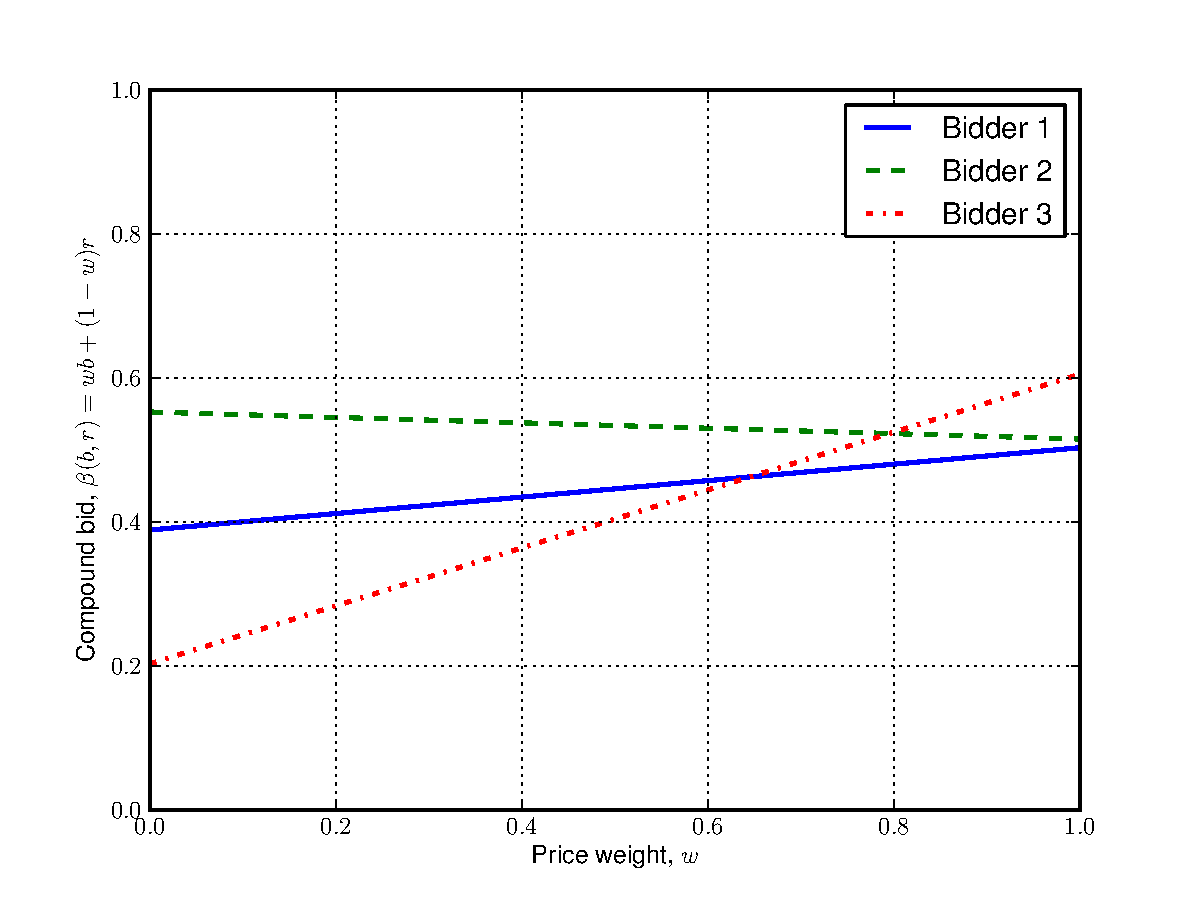
\includegraphics[width=\figsize]{2/Figures/bids_fpa}
	\label{fig:bids_fpa}
\end{figure}

\begin{figure}[htp]
	\caption{The empirical density function of the intersections (10,000 runs and 3 network operators)}
	\vspace{0.5cm}
	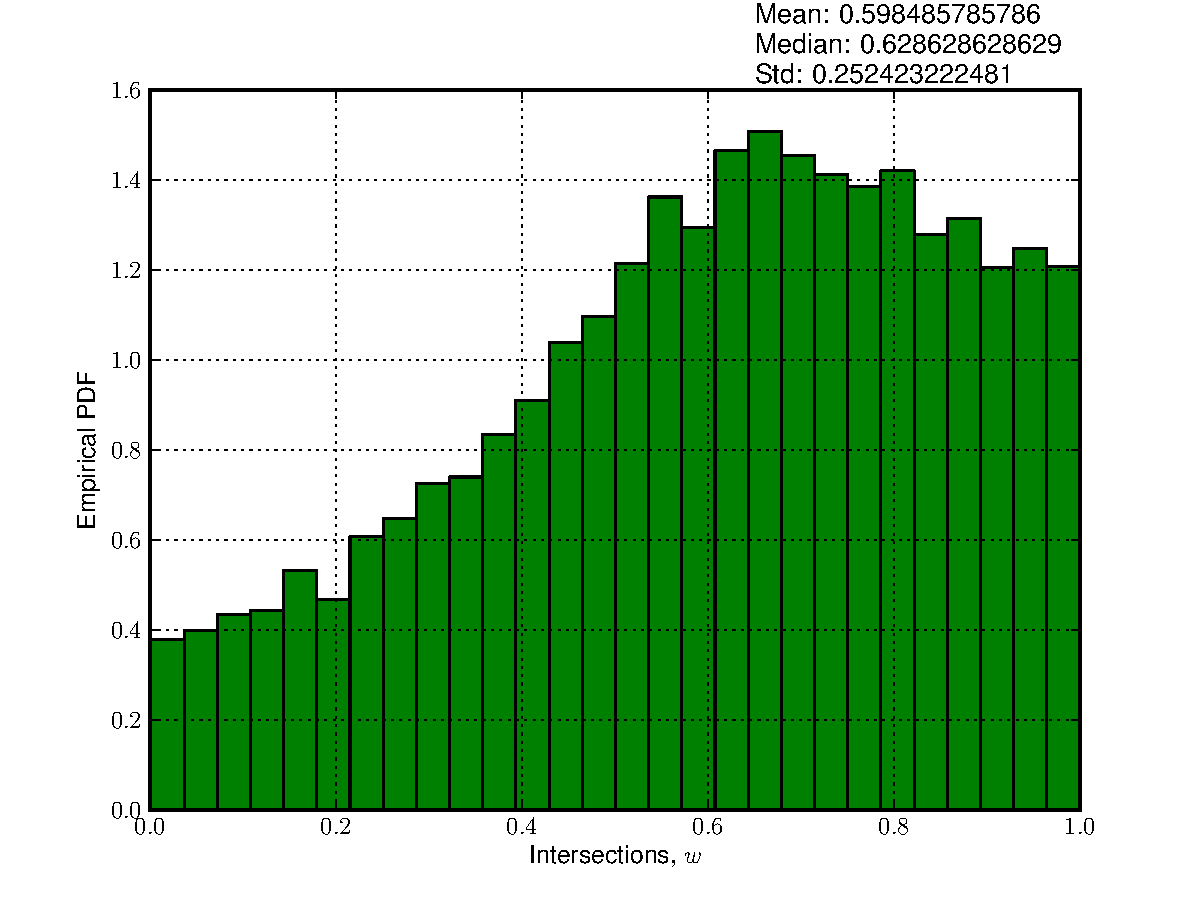
\includegraphics[width=\figsize]{2/Figures/hist_N_3}
	\label{fig:hist_N_3}
\end{figure}

\begin{figure}[hbp]
	\caption{The empirical probability distribution associated with the histogram in Figure~\ref{fig:hist_N_3}}
	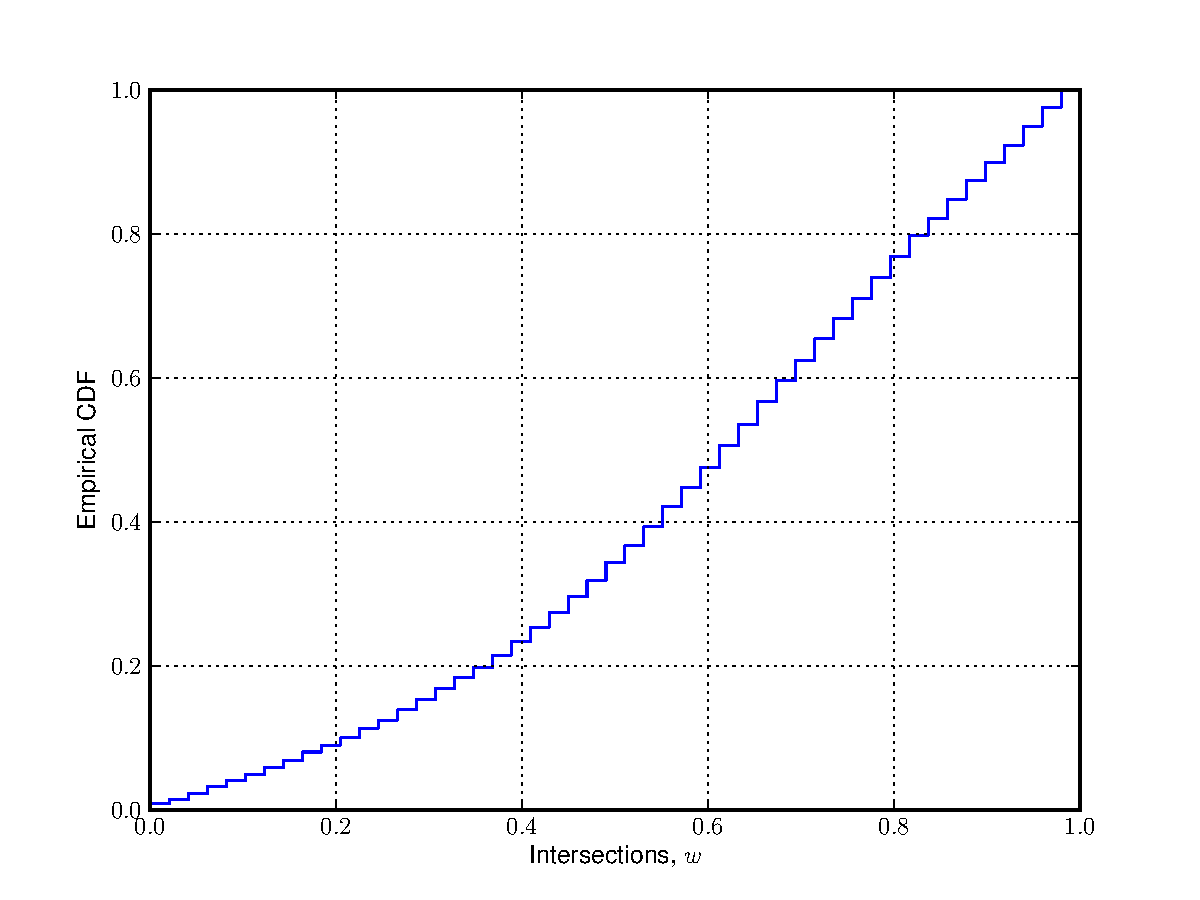
\includegraphics[width=\figsize]{2/Figures/ecdf_N_3}
	\label{fig:ecdf_N_3}
\end{figure}

Table~\ref{tab:bids_fpa} and Figure~\ref{fig:bids_fpa} depict a particular output from the simulation for $n=3$ network operators. In this particular example, for $w\in (0.65, 1]$, network operator 1 who is characterized by the lowest cost of all three network operators, wins the auction; that is, the network operator 1's compound bid is the lowest. At $w=0.65$, an intersection occurs of network operator 1's and 3's compound bids, and after that network operator 3 becomes the winner. If the simulation was repeated $r$ times, and the intersection was to fall within a close neighborhood of $w=0.65$ in the vast majority of cases, then $b^*$ could quite likely be an equilibrium bidding strategy in the interval $w\in (0.65, 1]$. This is predicated on the fact that, as $w\rightarrow 1$, the offered price dominates the value of the compound bid; that is, the offered price is weighted more than the reputation rating (Equation~\eqref{eq:def_beta}).

The methodology is as follows:
\begin{enumerate}
	\item Generate cost/reputation rating/bid triplet using the Monte Carlo methods.
	\item Find the winner for $w=1$, network operator $i$, say (in Figure~\ref{fig:bids_fpa} that would be network operator~1).
	\item Decrease the value of $w$ until network operator $i$ no longer wins, and save the value of $w$ for which that happens. Henceforth, such an event shall be denoted by $I$, and called \emph{the event when an intersection has occurred.}
	\item If the intersection did not occur, $I=0$, increase the counter that counts the frequency of such an event, and then discard that run.
	\item Repeat $r$ number of times.
\end{enumerate}

The case when $r=10,000$ runs, and $n=3$ network operators is depicted in the two figures: Figure~\ref{fig:hist_N_3} shows the empirical density function of the intersections; and Figure~\ref{fig:ecdf_N_3} depicts the empirical distribution function of the intersections. The probability of an intersection occurring equals $P\{I=1\} = 0.67$. It can be concluded from the figures that, on average, intersections occur at $\bar{w}=0.6$, which represents the mean of the distribution. However, the peak observed in a close neighborhood of $\bar{w}$ is not significant enough to conclude that bidding according to $b^*$ is the best strategy one can take for $w\in (\bar{w},1]$.

A more formal argument goes as follows. Figure~\ref{fig:ecdf_N_3} depicts the probability that an intersection has occurred within an interval $(-\infty,w]$ given that an intersection has occurred, $I=1$; that is, if the former event is denoted by $W$, then the figure describes $P\{W\in(-\infty, w] \mid I=1\}$. From this, the probability of winning for network operator $i$ (as defined in the listing above) given any $w$ is
\begin{align}
	&P\{\text{winning} \mid w\} \nonumber\\
	&= 1 - P\{W\in[w,\infty) \cap I=1\} \nonumber\\
	&= 1 - P\{W\in[w,\infty)\mid I=1\}P\{I=1\} \nonumber\\
	&= 1 - \left( 1 - P\{W\in(-\infty, w]\mid I=1\} \right)P\{I=1\}.
	\label{eq:mc_prob_winning}
\end{align}

In order to verify Equation~\eqref{eq:mc_prob_winning}, let $w\in\{0.25,0.75\}$ and run a Monte Carlo simulation which counts the number of times when the network operator with the lowest cost is the winner; i.e., the winner of the auction for $w=1$. When $w=0.25$, 
\begin{equation*}
	P\{\text{winning}\mid w=0.25\} = 1 - (1-0.13)0.67 = 0.4171
\end{equation*}
according to Equation~\eqref{eq:mc_prob_winning}, while the numerically obtained result 
\begin{equation*}
	P\{\text{winning}\mid w=0.25\} = 0.4136.
\end{equation*}
When $w=0.75$,
\begin{equation*}
	P\{\text{winning}\mid w=0.75\} = 1 -(1-0.68)0.67 = 0.7856
\end{equation*}
according to Equation~\eqref{eq:mc_prob_winning}, while the numerically obtained result
\begin{equation*}
	P\{\text{winning}\mid w=0.75\} = 0.7866.
\end{equation*}

Clearly, the prediction based on Equation~\eqref{eq:mc_prob_winning} converges to the numerically obtained result. Moreover, it is worth noting that for $w=0.25$, bidding according to $b^*$ guarantees the probability of winning for the network operator with the lowest cost of only $0.4171$ which is below $50\%$. Thus, the network operators will definitely deviate from $b^*$ for low values of $w$. On the other hand, for $w=0.75$, $b^*$ seems to achieve a relatively high probability of winning for the network operator with the lowest cost; i.e., the probability of $0.7856$. However, the argument is incomplete in the sense that it only considers the probability of winning rather than the expected utility.
% subsubsection special_case_w_1_ (end)

\subsubsection{Special Case $r_i=r_j$} % (fold)
\label{sub:special_case_r_i_r_j_}
In the last extreme case, when all network operators are characterized by the same reputation rating, i.e., when $r_i = r_j$ for all $i\neq j$, and when $w\neq 0$, it can be easily verified that the problem simplifies to the special case $w=1$. To see why, let $r = r_i,$ for all network operators $i$. Then, for all $i\in N$ and $w\neq 0$
\begin{align*}
	&\beta(b_i, r) < \min_{j\neq i} \beta(b_j, r)\\
	\iff &\frac{1}{w} \left(b_i + \frac{1-w}{w} r\right) < \frac{1}{w} \min_{j\neq i} \left(b_j + \frac{1-w}{w} r\right)\\
	\iff &b_i + \frac{1-w}{w} r < \min_{j\neq i} b_j + \frac{1-w}{w} r\\
	\iff &b_i < \min_{j\neq i} b_j.
\end{align*}
Hence, the utility of each network operator $i$ simplifies to
\begin{equation*}
	u_i(b,c,r) = \left\{
	\begin{array}{l l}
		b_i - c_i &\text{ if } b_i < \displaystyle\min_{j\neq i} b_j,\\
		0 &\text{ if } b_i > \displaystyle\min_{j\neq i} b_j.
	\end{array}
	\right.
\end{equation*}
Formally,
\begin{corollary}
\label{cor:special_case_r_i_r_j_}
Suppose $c_i$ is i.i.d.~over the interval $[0,1]$ for all $i\in N$ and $r_i\in [0,1]$ for all $i\in N$ is common knowledge. Suppose $r_i = r_j$ for all $i\neq j$, and $w\neq 0$. Then, the problem simplifies to the special case $w=1$, and hence, $b^*_{FPA}$ is the symmetric equilibrium bidding strategy (Proposition~\ref{prop:special_case_w_1}).
\end{corollary}
% subsection special_case_r_i_r_j_ (end)
% subsection generic_case (end)

\subsection{Restricted Case $n=2$} % (fold)
\label{sub:direct_restricted_case_n_2_}
In this section, we will restrict our attention to only two network operators. Since the problem in its generic form proved too complex to be solved analytically, this section will explore whether in a much simplified scenario it is possible to find a closed-form solution. To this end, let $n=2$. The utility function for each network operator $i\in N$ thus becomes
\begin{equation}
	\label{eq:utility_n_2}
	u_i(b,c,r) = \left\{
	\begin{array}{l l}
		b_i - c_i &\text{if } \beta(b_i,r_i) < \beta(b_j,r_j),\\
		\frac{1}{2}(b_i - c_i) &\text{if } \beta(b_i,r_i) = \beta(b_j,r_j),\\
		0 &\text{otherwise}.
	\end{array}\right.
\end{equation}
Furthermore, the assumption about the symmetric equilibrium profile is relaxed; that is, network operators are permitted to use differing bidding strategies.

The analysis is conducted in two steps. Firstly, it is assumed that information is complete; that is, that each network operator not only knows their own cost and reputation, but also those of their opponent's. Secondly, the standard case is considered; that is, that the reputation ratings of the network operators are assumed to be known, while the costs are private knowledge.

\subsubsection{Complete Information} % (fold)
\label{ssub:complete_information_n_2}
Here, we assume that information is complete; i.e., that each network operator knows their own and their opponent's cost and reputation. In total, there are 7 different bidding scenarios to consider.

\begin{figure}[htp]
	\caption{Different bidding scenarios for $r_i < r_j$}
	\label{fig:complete_N_2_1}
	\vspace{0.5cm}
	\begin{subfigure}[b]{0.5\textwidth}
	  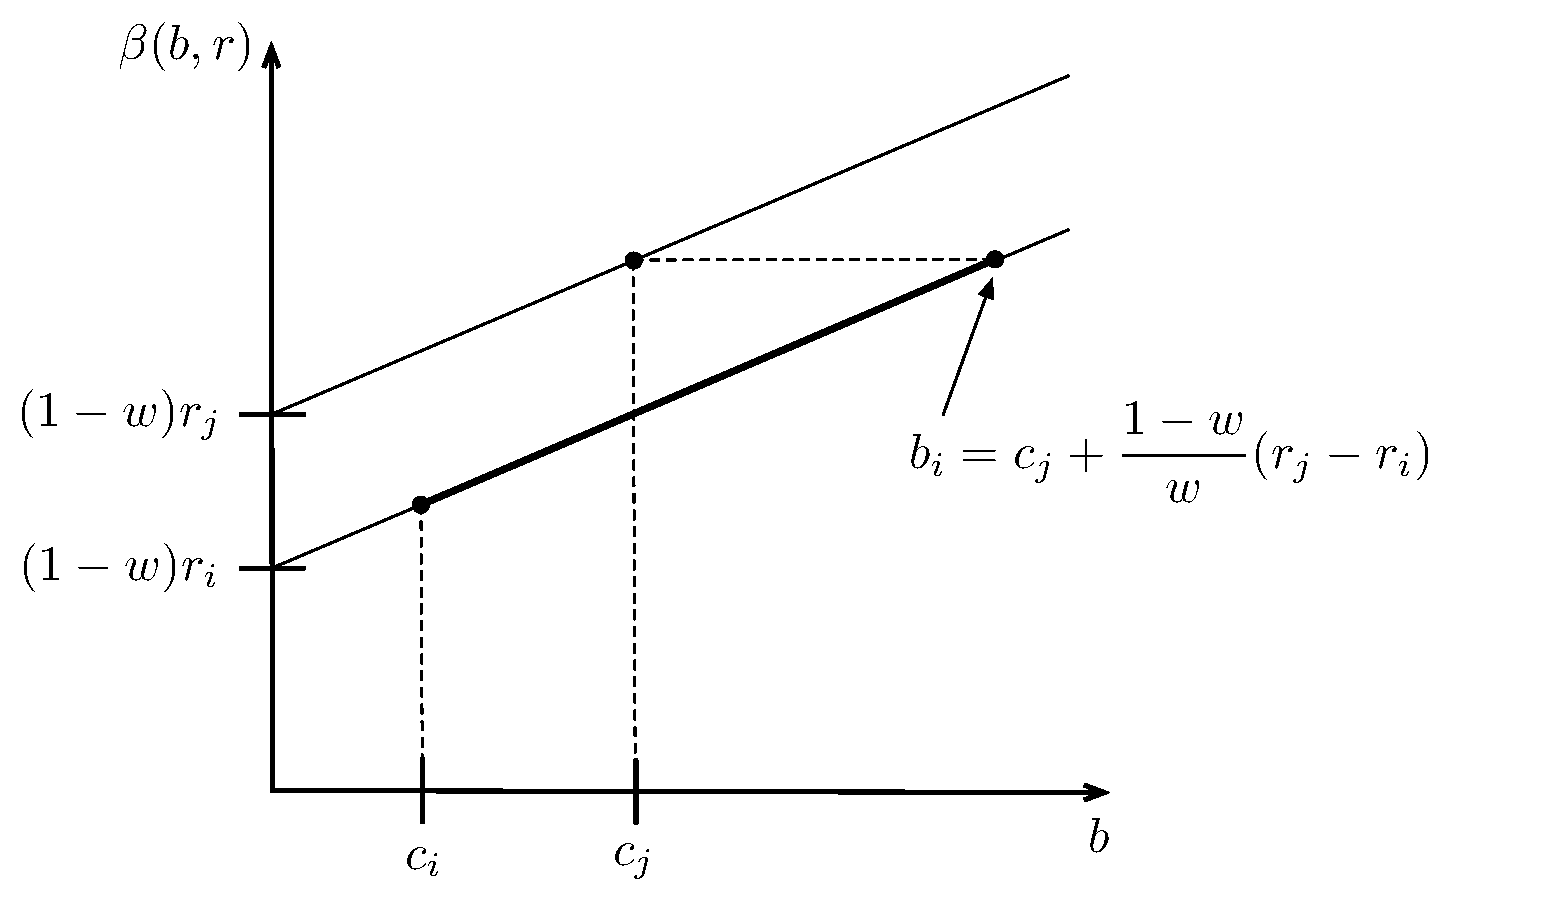
\includegraphics[width=2.8in]{2/Figures/complete_N_2_c1}
	  \caption{$c_i < c_j$}
	  \label{fig:complete_N_2_c1}
	\end{subfigure}
	\begin{subfigure}[b]{0.5\textwidth}
	  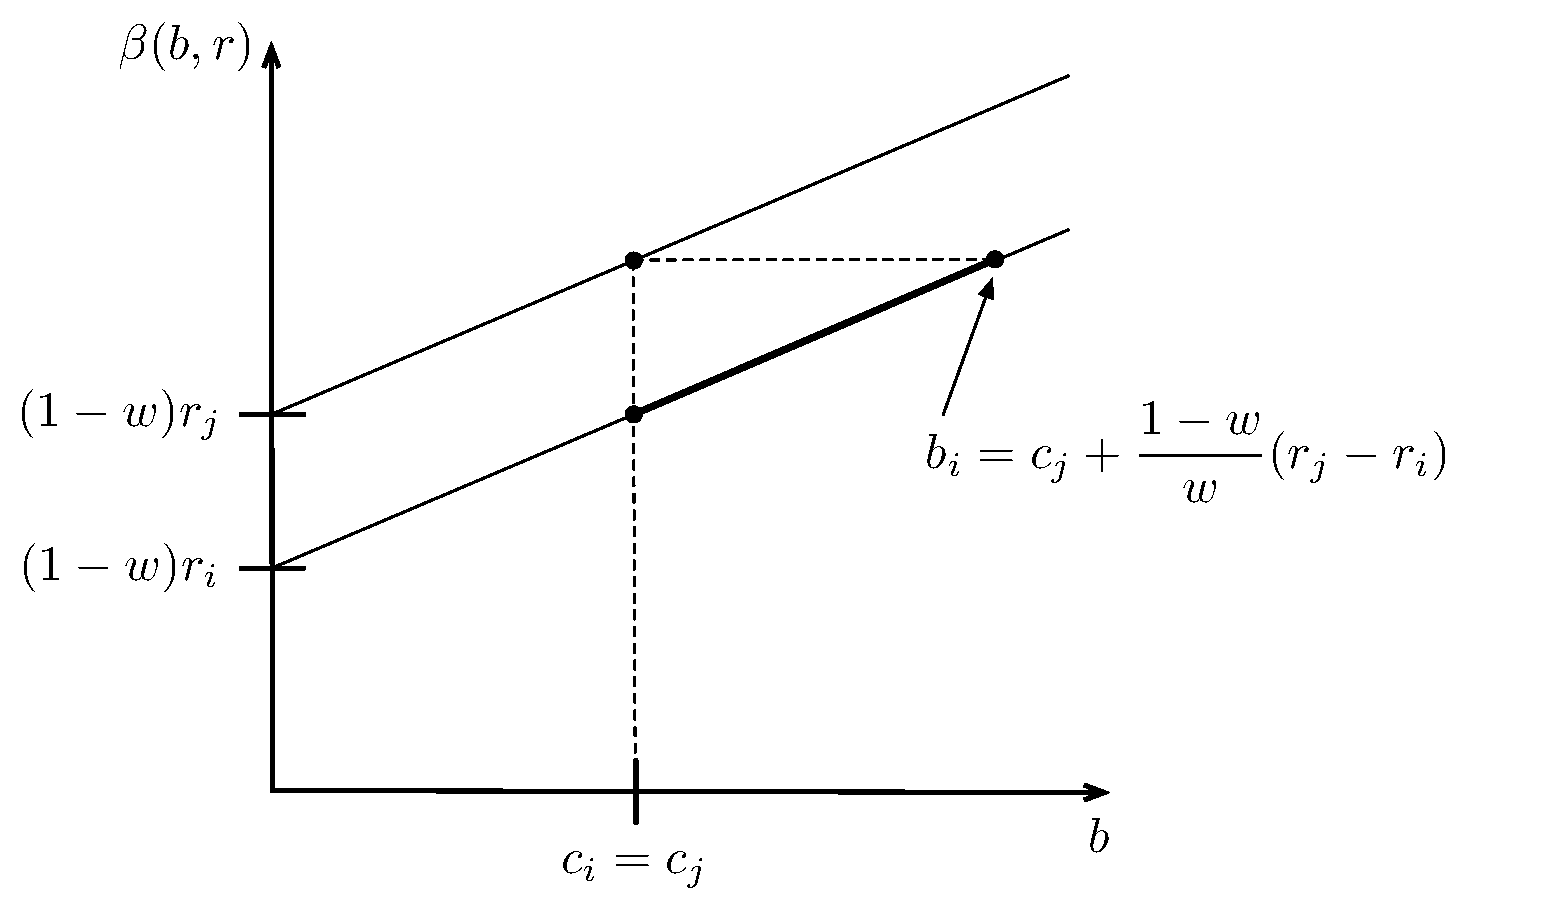
\includegraphics[width=2.8in]{2/Figures/complete_N_2_c2}
	  \caption{$c_i = c_j$}
	  \label{fig:complete_N_2_c2}
	\end{subfigure}
	\vspace{0.5cm}\\
	\begin{subfigure}[b]{0.5\textwidth}
	  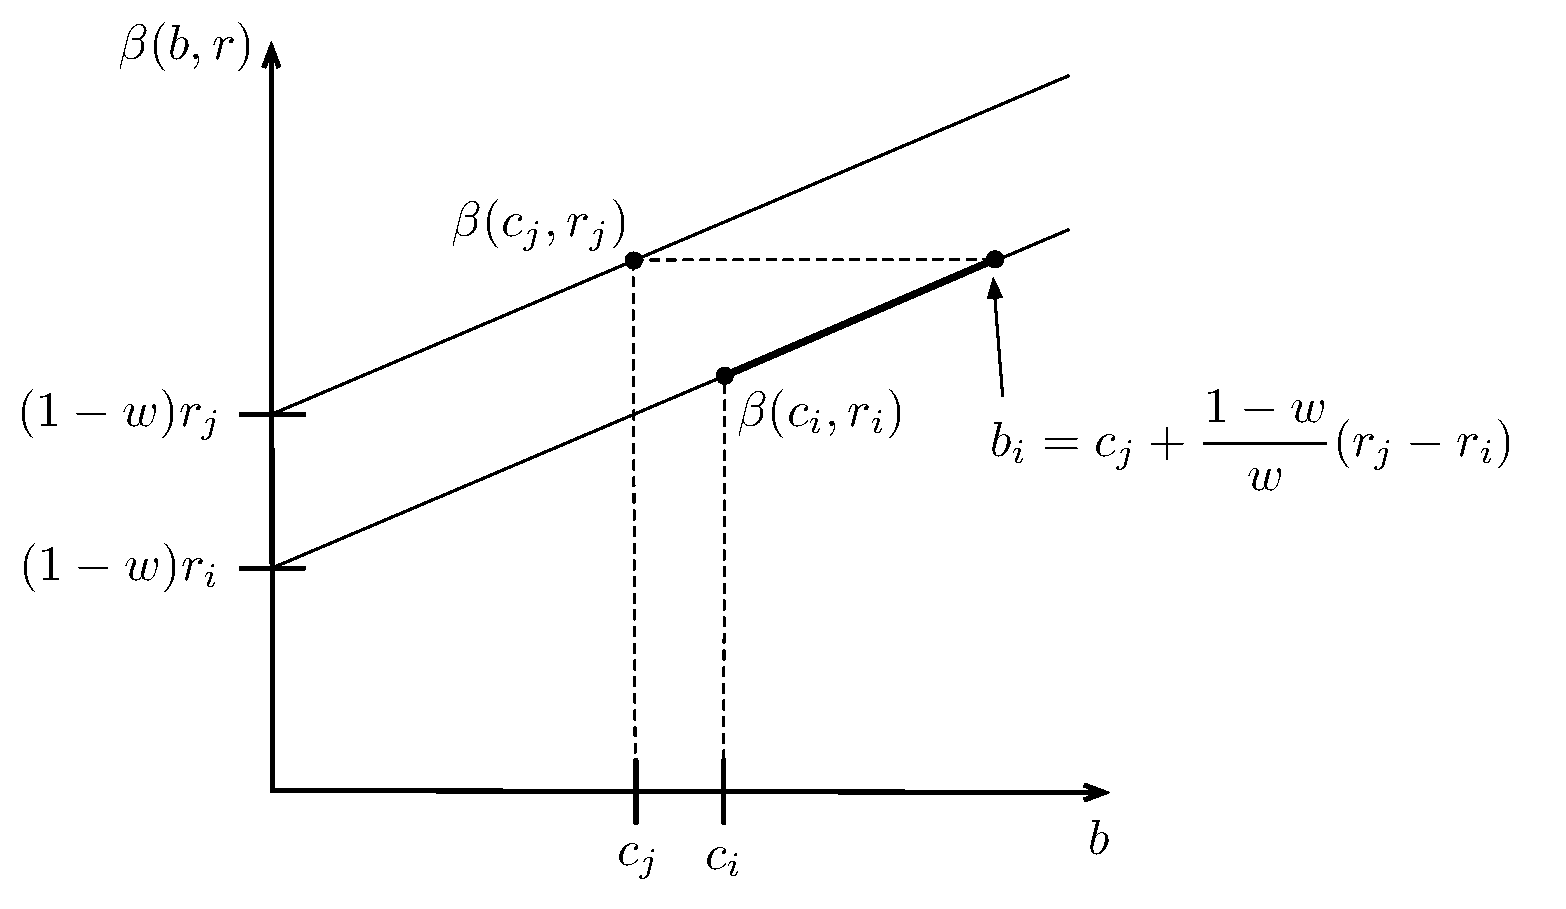
\includegraphics[width=2.8in]{2/Figures/complete_N_2_c3_1}
	  \caption{$c_i > c_j$ and $\beta(c_i,r_i) < \beta(c_j,r_j)$}
	  \label{fig:complete_N_2_c3_1}
	\end{subfigure}
	\begin{subfigure}[b]{0.5\textwidth}
	  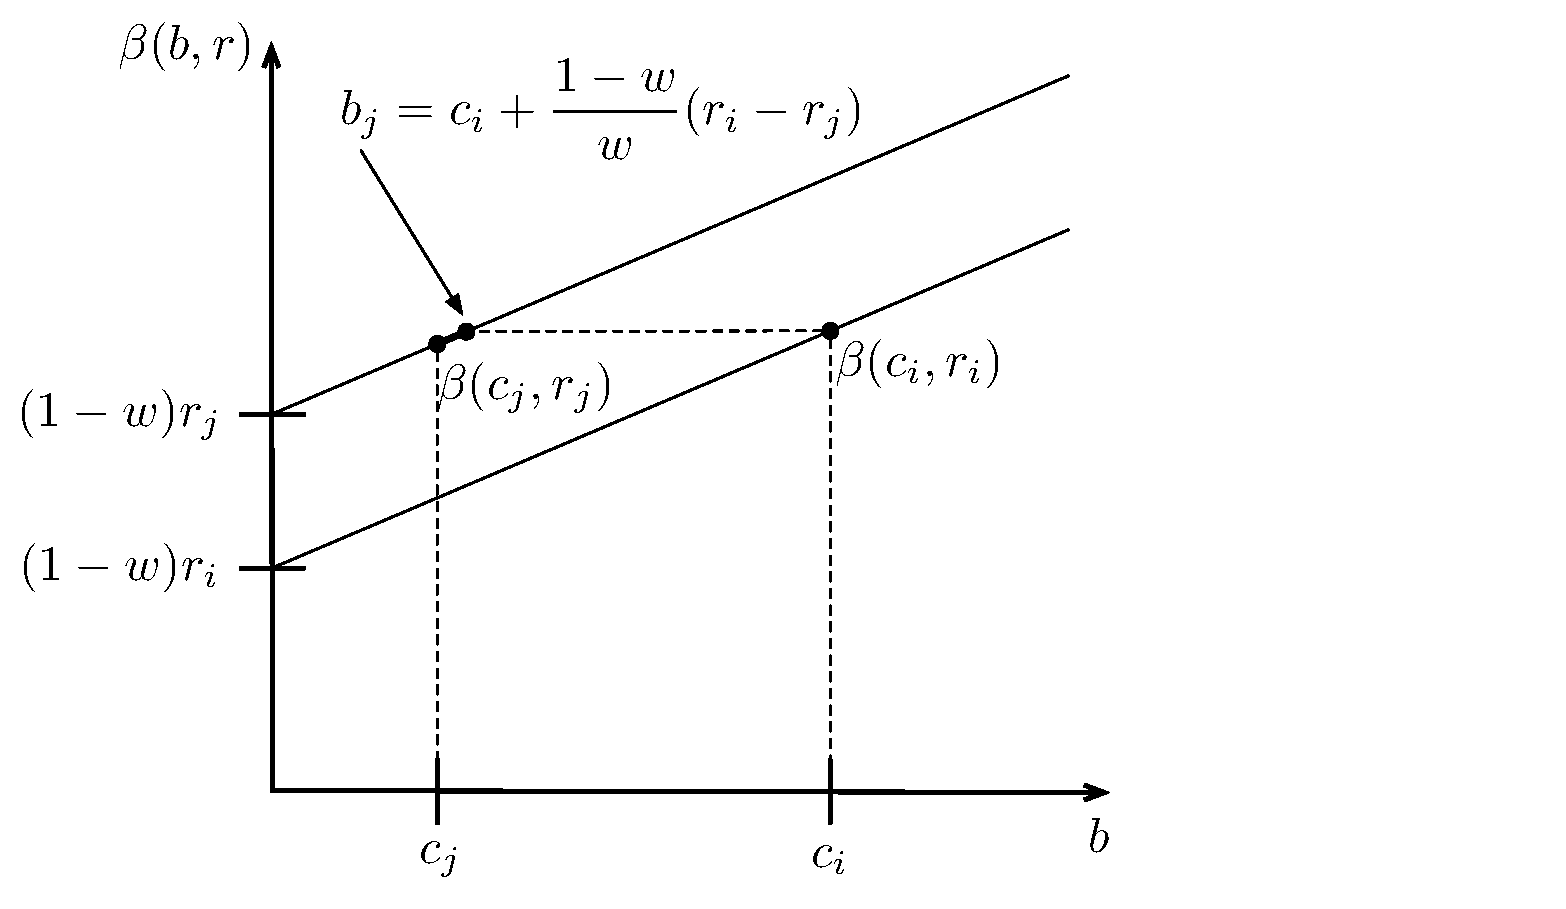
\includegraphics[width=2.8in]{2/Figures/complete_N_2_c3_2}
	  \caption{$c_i > c_j$ and $\beta(c_i,r_i) \ge \beta(c_j,r_j)$}
	  \label{fig:complete_N_2_c3_2}
	\end{subfigure}
\end{figure}

\begin{figure}[htp]
	\caption{Different bidding scenarios for $r_i = r_j$}
	\vspace{0.5cm}
	\begin{subfigure}[b]{0.5\textwidth}
		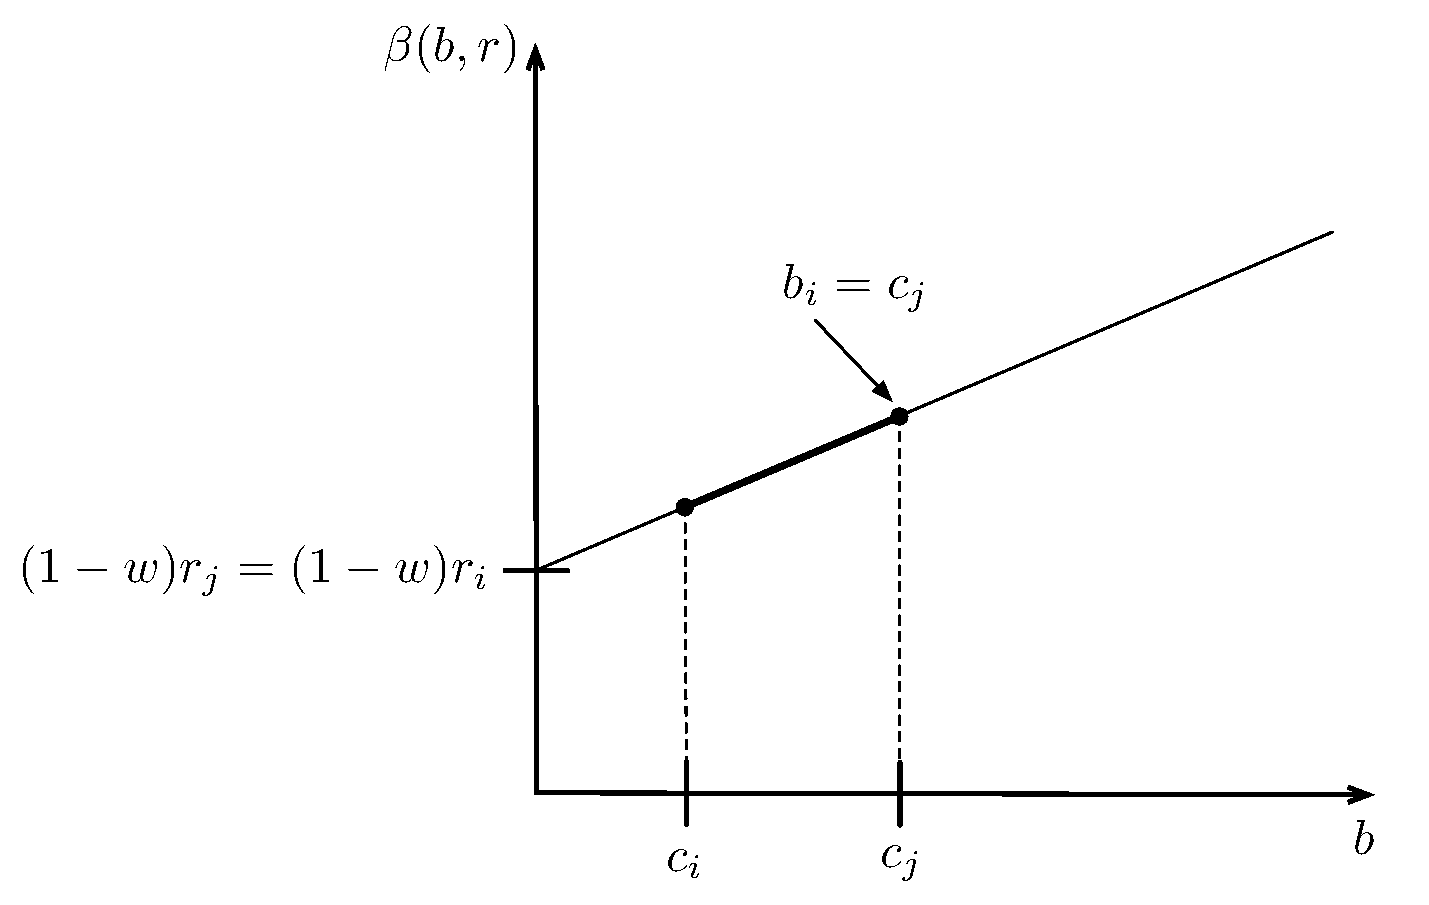
\includegraphics[width=2.8in]{2/Figures/complete_N_2_c4}	  
	  \caption{$c_i<c_j$}
	  \label{fig:complete_N_2_c4}
	\end{subfigure}
	\vspace{0.5cm}\\
	\begin{subfigure}[b]{0.5\textwidth}
	  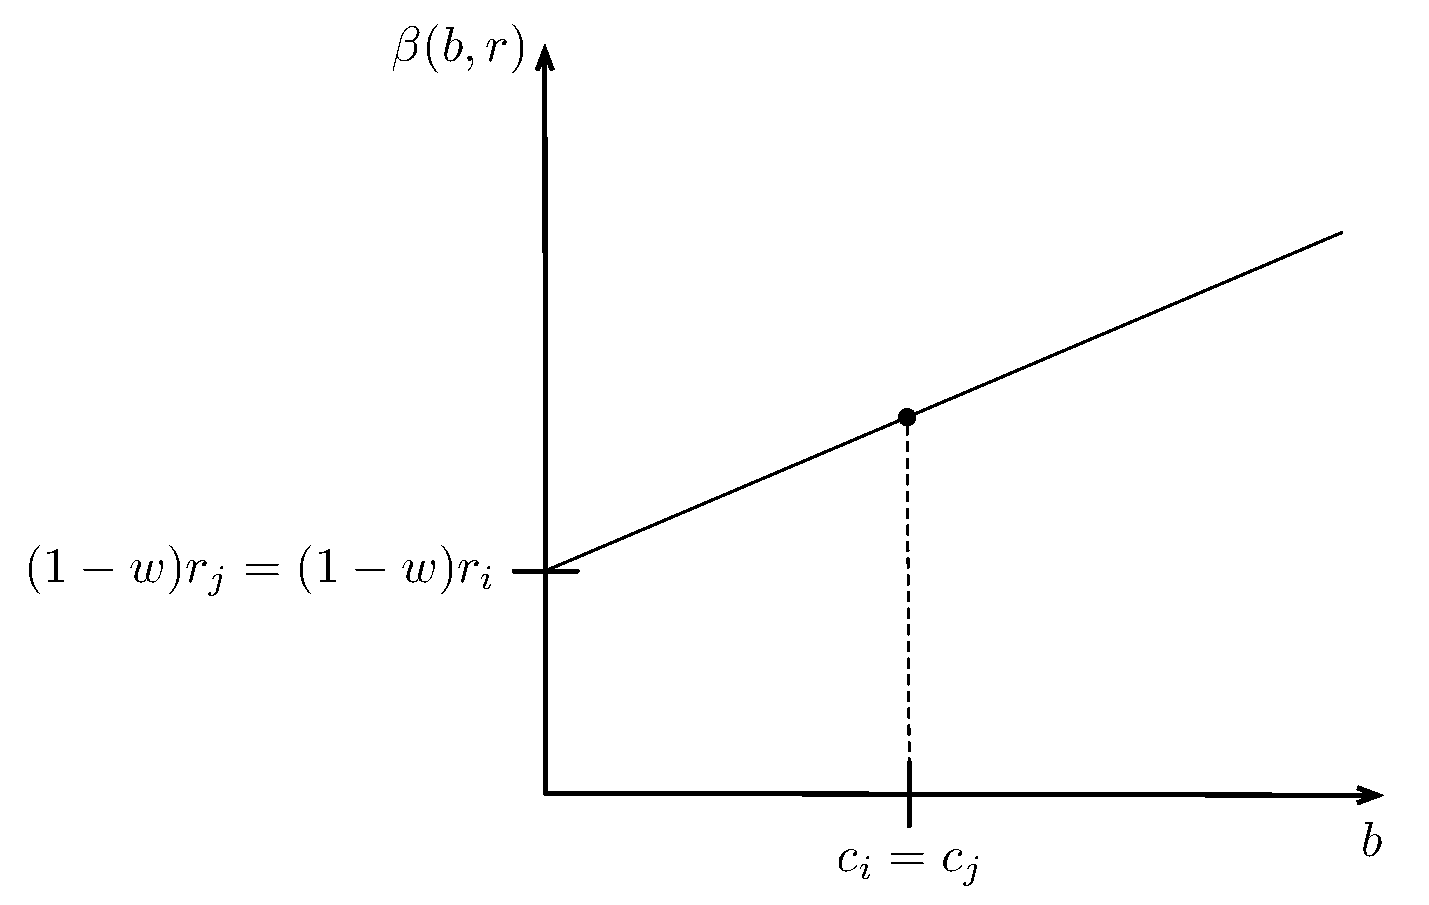
\includegraphics[width=2.8in]{2/Figures/complete_N_2_c5}
	  \caption{$c_i=c_j$}
	  \label{fig:complete_N_2_c5}
	\end{subfigure}
	\vspace{0.5cm}\\
	\begin{subfigure}[b]{0.5\textwidth}
	  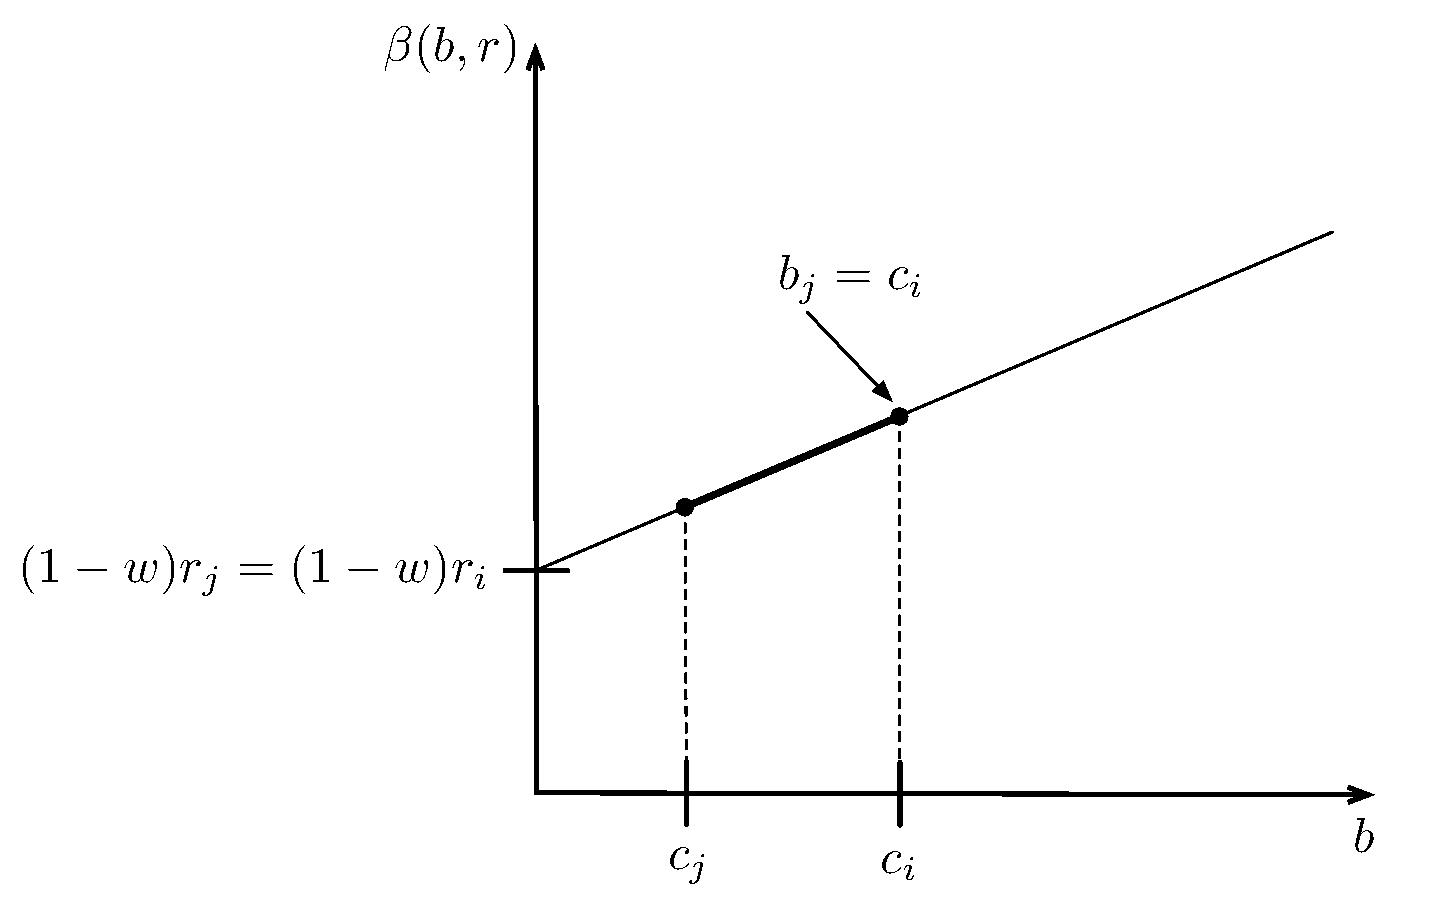
\includegraphics[width=2.8in]{2/Figures/complete_N_2_c6}
	  \caption{$c_i > c_j$}
	  \label{fig:complete_N_2_c6}
	\end{subfigure}
	\label{fig:complete_N_2_2}
\end{figure}

Figure~\ref{fig:complete_N_2_1} shows the first 4 cases for which $r_i < r_j$. (Note that exactly the same reasoning applies to the situation when $r_i > r_j$.) If $c_i < c_j$, network operator $i$ is guaranteed a victory and a positive profit as long as they bid within the highlighted part of the $\beta(b,r)$ curve depicted in Figure~\ref{fig:complete_N_2_c1}. Thus, their optimal bidding strategy would be to bid slightly less than their opponent's compound bid evaluated at their opponent's cost, $\beta(c_j,r_j)$; that is, $b_i = c_j + \frac{1-w}{w}(r_j-r_i) - \epsilon$ where $\epsilon>0$ is very small. Network operator $j$, on the other hand, should find it optimal to bid $b_j = c_j$. To see why, suppose network operator $j$ bids $\hat{b}_j>c_j$. Since network operator $i$'s reputation rating and cost are strictly lower than those of network operator $j$'s, they can undercut the network operator $j$'s bid by a small amount so that $\hat{b}_i < \hat{b}_j$ and still make positive profit. But, in response, network operator $j$ will find it optimal to lower their bid so that it undercuts that of network operator $i$'s; that is, $\hat{b}_j < \hat{b}_i$. This process will continue until one of the network operators is forced to bid their cost. Since network operator $i$'s reputation rating and cost are strictly lower than those of network operator $j$'s, we conclude that $b_j = c_j$ and $b_i = c_j + \frac{1-w}{w}(r_j-r_i) - \epsilon$ where $\epsilon>0$ is very small.

If $c_i = c_j$, arguing in the similar manner as previously, network operator $i$'s optimal bidding strategy would be to bid $b_i = c_j + \frac{1-w}{w}(r_j-r_i) - \epsilon$ where $\epsilon>0$ is very small; while network operator $j$ should bid $b_j = c_j$ (Figure~\ref{fig:complete_N_2_c2}).

If $c_i > c_j$, there are two cases to consider. If $\beta(c_i,r_i)<\beta(c_j,r_j)$, then network operator $i$ still has some room for maneuver, and should find it optimal to bid $b_i = c_j + \frac{1-w}{w}(r_j-r_i) - \epsilon$ where $\epsilon>0$ is very small; while network operator $j$ to bid $b_j=c_j$ (Figure~\ref{fig:complete_N_2_c3_1}). If $\beta(c_i,r_i)\ge \beta(c_j,r_j)$, on the other hand, the roles are reversed, and network operator $j$ should find it optimal to bid $b_j = c_i + \frac{1-w}{w}(r_i-r_j) - \epsilon$ where $\epsilon>0$ is very small; while network operator $i$ to bid $b_i = c_i$ (Figure~\ref{fig:complete_N_2_c3_2}).

Figure~\ref{fig:complete_N_2_2} depicts the remaining 3 cases for which $r_i=r_j$. If $c_i < c_j$, network operator $i$'s optimal bidding strategy would be to bid $b_i = c_j - \epsilon$ where $\epsilon>0$ is very small; while network operator $j$ should bid $b_j = c_j$ (Figure~\ref{fig:complete_N_2_c4}).

If $c_i = c_j$, both network operators should bid their costs; that is, $b_i = c_i$ and $b_j = c_j$ (Figure~\ref{fig:complete_N_2_c5}).

If $c_i > c_j$, network operator $j$'s optimal bidding strategy would be to bid $b_j = c_i - \epsilon$ where $\epsilon>0$ is very small; while network operator $i$ should bid $b_i = c_i$ (Figure~\ref{fig:complete_N_2_c6}).

It can be concluded that the bidding strategies depend only on costs if $r_i = r_j$. In the remaining cases, they are asymmetric in the sense that the winning network operator is characterized by
\begin{equation*}
	b_i = c_j + \frac{1-w}{w}(r_j - r_i) - \epsilon \quad\text{with }\epsilon>0\text{ being very small},
\end{equation*}
while the losing network operator by bidding their own cost
\begin{equation*}
	b_j = c_j.
\end{equation*}
Hence, when dealing with incomplete information, we will exploit these results by concentrating on equilibrium bidding strategies which are linear functions of cost.
% subsubsection complete_information_n_2 (end)

\subsubsection{Incomplete Information} % (fold)
\label{ssub:incomplete_information_n_2}
Here, we assume the standard case; that is, that reputation values for both network operators are known at the time of bidding; however, their costs are private knowledge. Suppose that the network operators use a strategy function $b_i: [0,1]\to\mathbb{R}$ defined by the rule
\begin{equation}
	\label{eq:pcomp_bidding_str}
	b_i(c_i) = m_i + n_i c_i,\quad\text{for all } m_i\in\mathbb{R},n_i>0,
\end{equation}
and costs are independently drawn from the uniform distribution over the interval $[0,1]$. In other words, (although somewhat counter-intuitive) we allow for negative bids from the network operators. The motivation for such an assumption will be explained in detail later on in the section. Note, moreover, that the strategy function is assumed to be linear in cost. Each network operator $i$ faces an optimization problem
\begin{equation}
	\label{eq:pcomp_exp_utility_uc}
	\max_{b_i}E \left[ b_i-c_i \:\middle\vert\: wb_i + (1-w)r_i < w(m_j + n_j C_j) + (1-w)r_j\right]
\end{equation}

If $w=0$, then the result described in Proposition~\ref{prop:special_case_w_0}, Section~\ref{ssub:special_case_w_0_}, holds. Otherwise, for $0<w\le 1$, each network operator $i$ solves
\begin{align}
	&\max_{b_i} E \left[ b_i-c_i \:\middle\vert\: \frac{1}{n_j}\left( b_i + \frac{1-w}{w}(r_i-r_j)-m_j \right) < C_j \right] \nonumber\\
	= &\max_{b_i}\int_{\frac{1}{n_j}(b_i + \frac{1-w}{w}(r_i-r_j)-m_j)}^{1} (b_i-c_i)dF_C(t)\nonumber\\
	= &\max_{b_i} \bigg(b_i-c_i\bigg) \left(1-\frac{1}{n_j}b_i-\frac{1}{n_j} \left(\frac{1-w}{w}(r_i-r_j)-m_j \right) \right).
	\label{eq:pcomp_exp_utility_w_1}
\end{align}
The first-order condition yields
\begin{align}
	&\qquad\quad 1 - \frac{2}{n_j}b_i + \frac{1}{n_j}c_i - \frac{1}{n_j}\left( \frac{1-w}{w}(r_i-r_j) - m_j \right) = 0 \nonumber\\
	&\iff b_i = \frac{n_j}{2} - \frac{1}{2}\left( \frac{1-w}{w}(r_i-r_j) - m_j \right) + \frac{1}{2}c_i.
\end{align}
(Note that the second-order condition is satisfied; i.e., $\frac{d^2}{db^2_i}E[\cdot\vert\cdot] = -\frac{2}{n_j} < 0$ since $n_j>0$.) Similar argument for network operator $j$ yields
\begin{equation}
	b_j = \frac{n_i}{2} - \frac{1}{2}\left( \frac{1-w}{w}(r_j-r_i) - m_i \right) + \frac{1}{2}c_j.
\end{equation}
Thus, it follows
\begin{equation*}
	\left\{
	\begin{array}{l l}
		n_i &= n_j = \displaystyle\frac{1}{2},\\[2ex]
		m_i &= \displaystyle\frac{n_j}{2} - \displaystyle\frac{1}{2}\left( \displaystyle\frac{1-w}{w}(r_i-r_j) - m_j \right),\\[2ex]
		m_j &= \displaystyle\frac{n_i}{2} - \displaystyle\frac{1}{2}\left( \displaystyle\frac{1-w}{w}(r_j-r_i) - m_i \right).
	\end{array}\right.
\end{equation*}
Solving the above equations simultaneously yields the equilibrium bidding strategy,
\begin{equation*}
	b_i'(c_i) = \frac{1}{2} - \frac{1-w}{3w}(r_i-r_j) + \frac{1}{2}c_i \quad\text{for all } i\in N.
\end{equation*}
Formally,
\begin{proposition}
\label{prop:pcomp_equi_bidding_str}
Let there be $n=2$ network operators. Suppose $c_i$ is independently drawn from uniform distribution over the interval $[0,1]$ for all $i\in N$, and $r_i\in [0,1]$ for all $i\in N$ is common knowledge. Then the equilibrium bidding strategy for all $w\in (0,1]$ is given by
\begin{equation}
	\label{eq:pcomp_equi_bidding_str}
	b_i'(c_i) = \frac{1}{2} - \frac{1-w}{3w}(r_i-r_j) + \frac{1}{2}c_i.
\end{equation}
\end{proposition}
\noindent Observe that the pair of strategies $(b_i', b_j')$ does not constitute a symmetric equilibrium.

\begin{table}[h]
	\caption{An exemplary set of cost-reputation pairs of two network operators}
	\vspace{0.5cm}
	\begin{tabular*}{0.5\columnwidth}[L]{@{\extracolsep{\fill}}r c c}
		\hlx{vhv}
		& \textbf{Cost}, $c_i$ & \textbf{Reputation rating}, $r_i$\\
		\hlx{vhv}
		\textbf{Network operator 1} & $0.75$ & $0.25$\\
		\textbf{Network operator 2} & $0.25$ & $0.75$\\
		\hlx{vhs}
	\end{tabular*}
	\label{tab:pcomp}
\end{table}

\begin{figure}[tp!]
	\caption{Compound bid plotted against the price weight}
	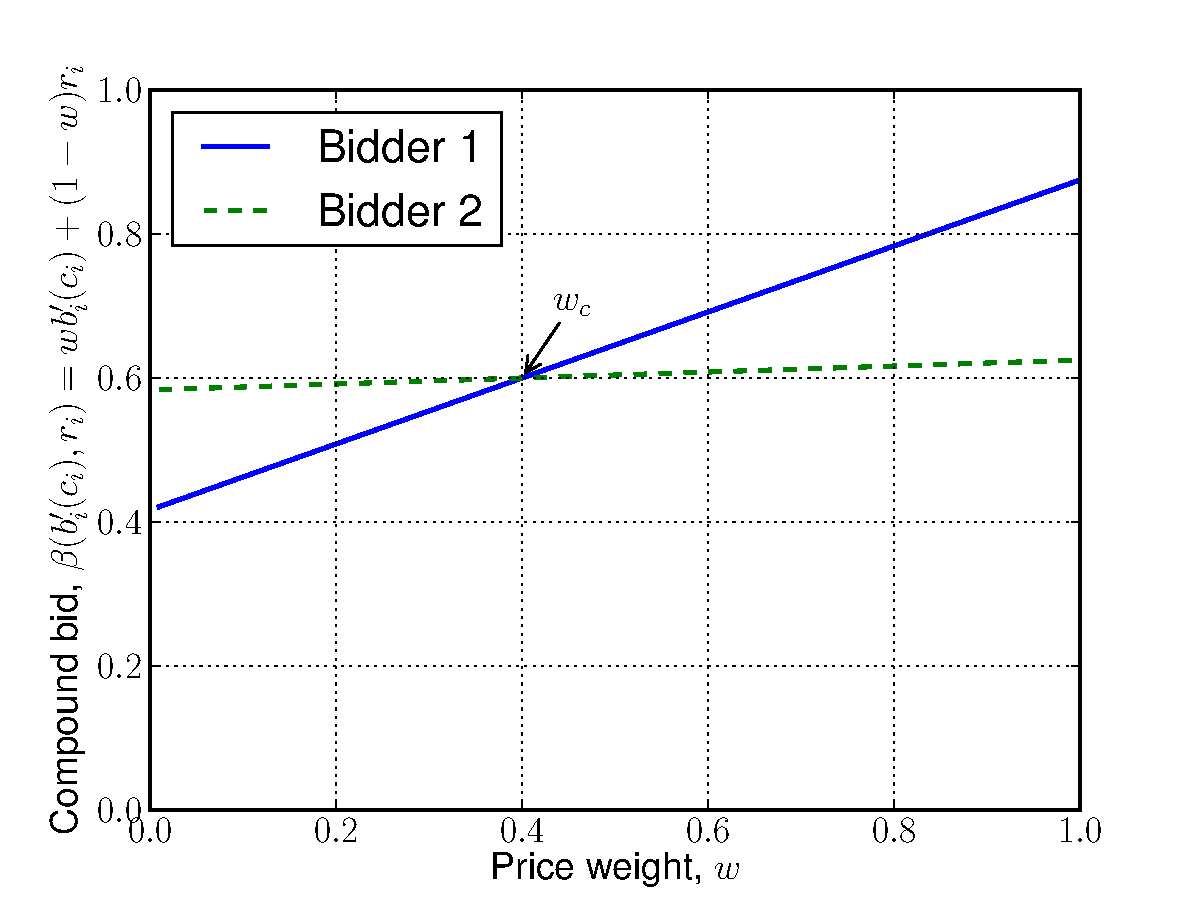
\includegraphics[width=\figsize]{2/Figures/pincomplete_bids_uc}
	\label{fig:pincomplete_bids_uc}
% \end{figure}
% \begin{figure}[bp!]
	\caption{Offered prices (bids) plotted against the price weight}
	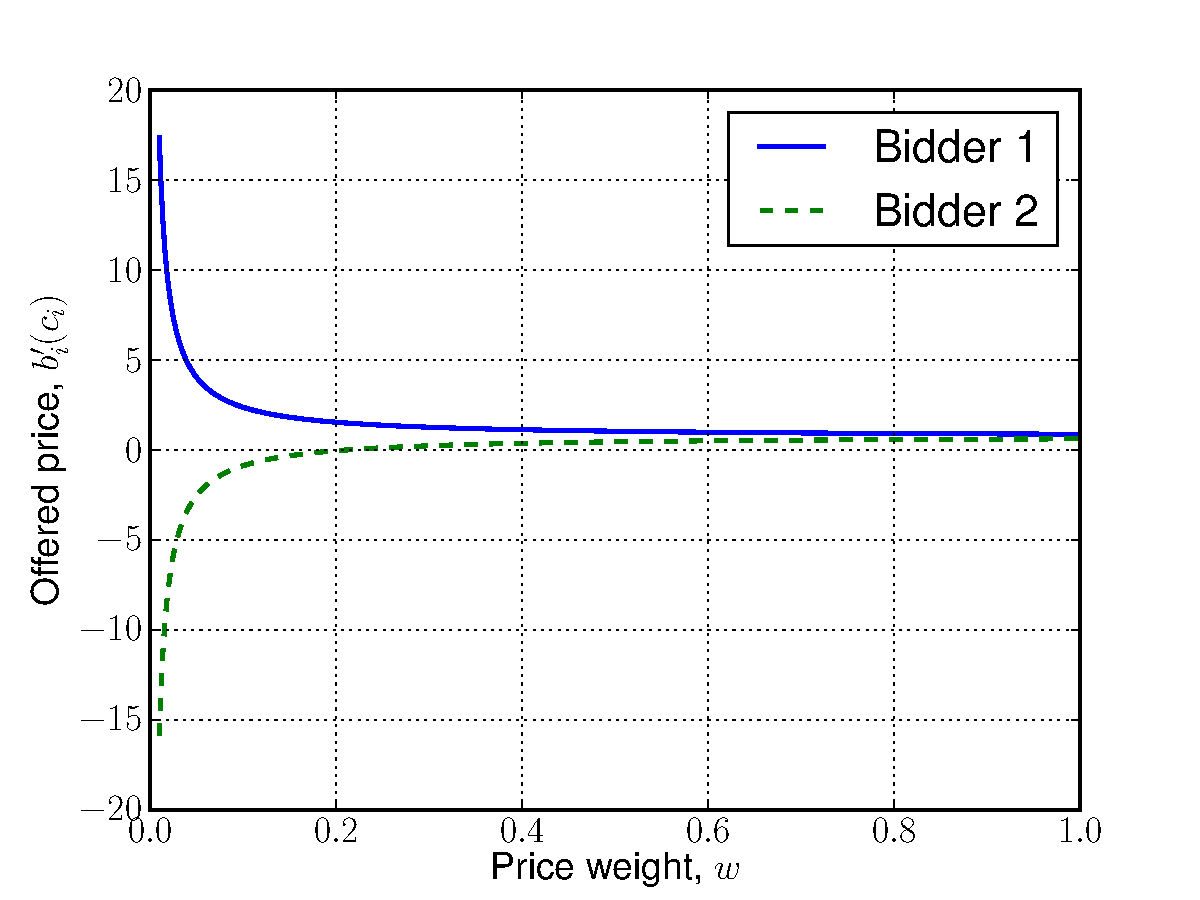
\includegraphics[width=\figsize]{2/Figures/pincomplete_prices_uc}
	\label{fig:pincomplete_prices_uc}
\end{figure}

By way of example, Table~\ref{tab:pcomp} depicts a particular set of cost-reputation pairs of two network operators. Figure~\ref{fig:pincomplete_bids_uc} shows the value of the compound bid, $\beta$, for different values of $w$ for both network operators, while Figure~\ref{fig:pincomplete_prices_uc} depicts the value of the monetary bid (or offered price), $b'_i$, for different values of $w$ for both network operators. The numerical data in Table~\ref{tab:pcomp} suggests that network operator 2 should be the winner for the values of $w\rightarrow 1$ since network operator 2's cost is strictly lower than that of their opponent's. On the other hand, network operator 1 should be winner for the values of $w\rightarrow 0$ since network operator 1's reputation rating is strictly lower than that of their opponent's (which implies that network operator 1's reputation is in fact strictly higher than that of their opponent's). This prediction agrees with the numerical output shown in Figure~\ref{fig:pincomplete_bids_uc}. Let $w_c$ denote the value of $w$ for which an intersection between the compound bids of both network operators occurs (if it exists). In Figure~\ref{fig:pincomplete_bids_uc}, $w_c=0.4$. Hence, network operator 2 wins the auction for the values of $w\in(w_c,1]$, while network operator 1 for the values of $w\in[0,w_c)$. Note, moreover, that network operator 2 bids below their cost for values of $w<w_c$ (Figure~\ref{fig:pincomplete_prices_uc}). However, this does not necessarily disqualify the equilibrium bidding strategies given by Equation~\eqref{eq:pcomp_equi_bidding_str}. The following observations show why.

Firstly,
\begin{proposition}
\label{prop:pcomp_negative_bids}
Suppose both network operators bid according to $b_i'$ bidding strategies. Then they are guaranteed nonnegative profit in case of winning (or a draw).
\end{proposition}
\noindent Even though the prediction suggests that one of the network operators may bid negatively, they will not win the auction, and hence, are guaranteed profit at worst equal to zero.

Secondly, let $(\mathbf{Q},\mathbf{M})$ be the direct mechanism induced by the equilibrium bidding strategies, $b_i'$, in Equation~\eqref{eq:pcomp_equi_bidding_str} where $\mathbf{Q}=(Q_i,Q_j)$ and $\mathbf{M}=(M_i,M_j)$. Here, $Q_i$ represents the allocation rule defined by
\begin{equation}
	\label{eq:pcomp_allocation_rule}
	Q_i(c_i,c_j) =
	\left\{
	\begin{array}{l l}
		1 &\text{if } \beta(b_i'(c_i),r_i) < \beta(b_j'(c_j),r_j)\\
		\frac{1}{2} &\text{if } \beta(b_i'(c_i),r_i) = \beta(b_j'(c_j),r_j)\\
		0 &\text{otherwise}
	\end{array}
	\right.,
\end{equation}
while $M_i$ is the payment rule defined by
\begin{equation}
	\label{eq:pcomp_payment_rule}
	M_i(c_i,c_j) = Q_i(c_i,c_j)b_i'(c_i).
\end{equation}
Suppose network operator $j$ reveals their cost truthfully. The equilibrium payoff function for network operator $i$ characterized by cost $c_i$ but revealing $\hat{c}_i$ is
\begin{align}
	\tilde{\tilde{u}}_i(\hat{c}_i) &= E\left[ M_i(\hat{c}_i,C_j) - c_iQ_i(\hat{c}_i,C_j) \right]\nonumber \\
	&= E\left[ (b_i'(\hat{c}_i)-c_i)Q_i(\hat{c}_i,C_j) \right]\nonumber \\
	&= E\left[ b_i'(\hat{c}_i)-c_i \:\middle\vert\: \beta(b_i'(\hat{c}_i),r_i) < \beta(b_j'(C_j),r_j) \right].
	\label{eq:pcomp_expected_utility}
\end{align}
It turns out that it is in network operator $i$'s best interest to reveal their cost truthfully as well; i.e., $\hat{c}_i=c_i$. Moreover, both network operators cannot be better off by not participating in the auction; i.e., their equilibrium payoff function is nonnegative, $\tilde{\tilde{u}}_i(c_i)\ge 0$. Formally,
\begin{proposition}
\label{prop:pcomp_direct_mechanism}
The direct mechanism $(\mathbf{Q},\mathbf{M})$ where $\mathbf{Q}=(Q_i,Q_j)$ and $\mathbf{M}=(M_i,M_j)$ (with $Q_i$ and $M_i$ defined in Equations~\eqref{eq:pcomp_allocation_rule} and \eqref{eq:pcomp_payment_rule} respectively) satisfies both the IC and IR constraints.
\end{proposition}

Thirdly, suppose that economic agents are computers who bid on behalf of the network operators. This assumption is reasonable since there currently are estimated 6.1 billion mobile subscribers around the world \cite{Ericsson2011}. In other words, bidding on a per call basis would have to be automated by the network operators in order to make the process manageable. One way of achieving such an automation would be to utilize the concept of a direct mechanism. In a direct mechanism, economic agents submit their costs (which need not be truthful) directly to the mechanism which then computes the bids and chooses the winner on their behalf. By the Revelation Principle (which is stated in Section~\ref{sub:notation_mechanism_design_theory}), we know that for every mechanism and an equilibrium for that mechanism, there exists an incentive compatible direct mechanism which yields the same outcomes as in the given equilibrium of the original mechanism. In our case, the direct mechanism $(\mathbf{Q},\mathbf{M})$ is the direct representation of the DMP variant of an FPA. Since it is incentive compatible, economic agents will not lie about their costs. Since it is individually rational, they will find it beneficial to participate in the mechanism. Therefore, the possibility of one of the network operators bidding below their cost or negatively will not matter to any of the network operators and will not lead to an outcome in which the service is sold for a negative price.

Nonetheless, the possibility of one of the network operators bidding below their cost or negatively might seem counter-intuitive and irrational. The most straightforward solution is to constrain the original optimization problem in Equation~\eqref{eq:pcomp_exp_utility_uc}; that is, each network operator $i$ tries to solve for all $w\neq 0$
\begin{align}
	\label{eq:pcomp_exp_utility_c}
	&\max_{b_i}E \left[ b_i-c_i \:\middle\vert\: wb_i + (1-w)r_i < w(m_j + n_j C_j) + (1-w)r_j\right]\\
	&\text{subject to}\quad c_i-b_i\le 0.\nonumber
\end{align}
The constraint $c_i-b_i\le 0$ ensures that each network operator bids above or equal to their cost. However, this problem is much more complicated than its unconstrained version in Equation~\eqref{eq:pcomp_exp_utility_uc}. Not only is it necessary to solve the nonlinear constrained optimization problem for each network operator $i$, but also it needs to be done simultaneously \cite{Griffin2011}. To better explore the inherent complexity of the problem, we will apply the Karush-Kuhn-Tucker Conditions theorem (which is stated in Section~\ref{sub:notation_optimisation_theory}), and try to derive the equilibrium bidding strategies for all network operators. But first, note that, since $n_j>0$ ($n_i>0$ for network operator $j$), $E[\cdot \vert \cdot]$ is a concave function of $b_i$ ($b_j$ for network operator $j$). Moreover, the constraint as a function of $b_i$ ($b_j$ for network operator $j$) is affine, and hence convex. Therefore, the Karush-Kuhn-Tucker Conditions are necessary and sufficient conditions for a solution in nonlinear constrained optimization problem to be optimal.

The problem will be approached as follows. First, we will fix the bidding strategy for network operator $j$ and treat the problem as a standard nonlinear constrained optimization problem for network operator $i$. The same stage will be repeated for network operator $j$. Then the results of both stages will be combined together and solved simultaneously. In effect, this will result in derivation of the equilibrium bidding strategies for both network operators.

The Lagrangian of the problem for network operator $i$ is
\begin{align}
	&L_i(b_i,\lambda_i) \nonumber\\
	&= E \left[ b_i-c_i \:\middle\vert\: wb_i + (1-w)r_i < w(m_j + n_j C_j) + (1-w)r_j\right] - \lambda_i(c_i-b_i) \nonumber\\
	&= (b_i-c_i)\left(1-\frac{1}{n_j}b_i - \frac{1}{n_j}\left(\frac{1-w}{w}(r_i-r_j)-m_j\right)\right) - \lambda_i(c_i-b_i).
	\label{eq:pcomp_langrangean_bidder_i}
\end{align}
We look for stationary values of the Lagrangian, $L_i(b_i,\lambda_i)$, that satisfy the complementary slackness conditions. The first-order condition for stationarity is
\begin{align*}
	\frac{\partial L_i(b_i,\lambda_i)}{\partial b_i} &= \left( 1 - \frac{1}{n_j}b_i - \frac{1}{n_j}\left( \frac{1-w}{w}(r_i-r_j)-m_j \right) \right) + \frac{1}{n_j}\left(c_i-b_i\right) + \lambda_i\nonumber\\
	&=0,
\end{align*}
while the complementary slackness conditions are
\begin{equation*}
	\left\{
	\begin{array}{ll}
		&c_i-b_i\le 0,\\
		&\lambda_i\ge 0,\\
		&\lambda_i(c_i-b_i) = 0.
	\end{array}
	\right.
\end{equation*}
Therefore, there are two possible solutions to the problem for network operator $i$: $\lambda_i > 0$, and $\lambda_i=0$. In the first case, $\lambda_i > 0$ implies $b_i = c_i$ and
\begin{equation*}
	\lambda_i = \frac{1}{n_j}c_i + \frac{1}{n_j}\left( \frac{1-w}{w}(r_i-r_j) - m_j \right) - 1 > 0.
\end{equation*}
In the second case, $\lambda_i = 0$ implies
\begin{equation*}
	1 - \frac{1}{n_j}b_i - \frac{1}{n_j}\left( \frac{1-w}{w}(r_i-r_j) - m_j \right) - (b_i-c_i)\frac{1}{n_j} = 0.
\end{equation*}

Similarly, the Lagrangian of the problem for network operator $j$ is 
\begin{align}
	&L_j(b_j,\lambda_j) \nonumber\\
	&= E \left[ b_j-c_j \:\middle\vert\: wb_j + (1-w)r_j < w(m_i + n_i C_i) + (1-w)r_i\right] - \lambda_j(c_j-b_j) \nonumber\\
	&= (b_j-c_j)\left(1-\frac{1}{n_i}b_j - \frac{1}{n_i}\left(\frac{1-w}{w}(r_j-r_i)-m_i\right)\right) - \lambda_j(c_j-b_j).
	\label{eq:pcomp_langrangean_bidder_j}
\end{align}
The first-order condition for stationarity is
\begin{align*}
	\frac{\partial L_j(b_j,\lambda_j)}{\partial b_j} &= \left( 1 - \frac{1}{n_i}b_j - \frac{1}{n_i}\left( \frac{1-w}{w}(r_j-r_i)-m_i \right) \right) + \frac{1}{n_i}\left(c_j-b_j\right) + \lambda_j\nonumber\\
	&=0,	
\end{align*}
while the complementary slackness conditions are
\begin{equation*}
	\left\{
	\begin{array}{ll}
		&c_j-b_j\le 0,\\
		&\lambda_j\ge 0,\\
		&\lambda_j(c_j-b_j) = 0.
	\end{array}
	\right.	
\end{equation*}
Therefore, there are two possible solutions to the problem for network operator $j$: $\lambda_j > 0$, and $\lambda_j=0$. In the first case, $\lambda_j > 0$ implies $b_j=c_j$ and
\begin{equation*}
	\lambda_j = \frac{1}{n_i}c_j + \frac{1}{n_i}\left( \frac{1-w}{w}(r_j-r_i) - m_i \right) - 1 > 0.
\end{equation*}
In the second case, $\lambda_j=0$ implies
\begin{equation*}
	1 - \frac{1}{n_i}b_j - \frac{1}{n_i}\left( \frac{1-w}{w}(r_j-r_i) - m_i \right) - (b_j-c_j)\frac{1}{n_i} = 0.
\end{equation*}

Without loss of generality, suppose $r_i<r_j$. In total, there are four possible solutions to the simultaneous optimization problem: $\lambda_i=\lambda_j=0$; $\lambda_i > 0$ and $\lambda_j=0$; $\lambda_i=0$ and $\lambda_j > 0$; and $\lambda_i > 0$ and $\lambda_j > 0$.

Firstly, suppose $\lambda_i > 0$ and $\lambda_j > 0$. This implies $b_i=c_i$ and $b_j=c_j$. Hence, $n_i=n_j=1$ and $m_i=m_j=0$ which yields
\begin{equation*}
	\left\{
	\begin{array}{ll}
		\lambda_i &= c_i + \displaystyle\frac{1-w}{w}(r_i-r_j)-1,\\[2ex]
		\lambda_j &= c_j + \displaystyle\frac{1-w}{w}(r_j-r_i)-1.
	\end{array}
	\right.
\end{equation*}
But, since $r_i < r_j$, $\lambda_i < 0$ for all $c_i\in[0,1]$ and $w\in(0,1]$. Therefore, the case where $b_i=c_i$ and $b_j=c_j$ cannot constitute an equilibrium.

Secondly, suppose $\lambda_i=\lambda_j=0$. In this case, the problem is equivalent to the unconstrained optimization problem in Equation~\eqref{eq:pcomp_exp_utility_uc}. That is, we need to solve
\begin{equation*}
	\left\{
	\begin{array}{ll}
		1 - \displaystyle\frac{1}{n_j}b_i - \displaystyle\frac{1}{n_j}\left( \displaystyle\frac{1-w}{w}(r_i-r_j) - m_j \right) - (b_i-c_i)\displaystyle\frac{1}{n_j} &= 0,\\[2ex]
		1 - \displaystyle\frac{1}{n_i}b_j - \displaystyle\frac{1}{n_i}\left( \displaystyle\frac{1-w}{w}(r_j-r_i) - m_i \right) - (b_j-c_j)\displaystyle\frac{1}{n_i} &= 0.
	\end{array}
	\right.
\end{equation*}
This yields the bidding strategies as in Equation~\eqref{eq:pcomp_equi_bidding_str}; that is,
\begin{equation*}
	\left\{
	\begin{array}{ll}
		b_i'(c_i) &= \displaystyle\frac{1}{2} - \displaystyle\frac{1-w}{3w}(r_i-r_j) + \displaystyle\frac{1}{2}c_i,\\[2ex]
		b_j'(c_j) &= \displaystyle\frac{1}{2} - \displaystyle\frac{1-w}{3w}(r_j-r_i) + \displaystyle\frac{1}{2}c_j.
	\end{array}
	\right.
\end{equation*}
Since $r_i < r_j$, then
\begin{equation*}
	c_i - b_i'(c_i) = \frac{1}{2}c_i - \frac{1}{2} + \frac{1-w}{3w}(r_i-r_j) \le 0
\end{equation*}
for all $c_i\in[0,1]$ and $w\in(0,1]$. However, the same is not true for network operator $j$. Let
\begin{align*}
	c_j - b_j'(c_j) = 0 &\iff c_j = \frac{1}{2} - \frac{1-w}{3w}(r_j-r_i) + \frac{1}{2}c_j\\[2ex]
	&\iff w(c_j) = \frac{1}{1 + \frac{3}{2}\frac{1-c_j}{r_j-r_i}}.
\end{align*}
Since $r_i < r_j$ and $c_j\in[0,1]$, $w(c_j)\in(0,1]$. Hence, the constraint is satisfied for network operator $j$ as long as
\begin{equation*}
	c_j-b_j'(c_j) \le 0 \iff w \ge w(c_j).
\end{equation*}
In other words, for $w\ge w(c_j)$, $(b_i',b_j')$ constitutes an equilibrium of the constrained optimization problem in Equation~\eqref{eq:pcomp_exp_utility_c}. However, for $w < w(c_j)$, $(b_i', b_j')$ is no longer an equilibrium.

Therefore, for $w < w(c_j)$, the only alternative for network operator $j$ is to bid $b_j''(c_j)=c_j$. If network operator $i$ would continue to use the strategy $b_i'$ in Equation~\eqref{eq:pcomp_equi_bidding_str}, the complementary slackness conditions for network operator $j$ are satisfied; that is, for all $c_j\in[0,1]$
\begin{equation*}
	\lambda_j = 2(c_j - 1) + \frac{4}{3}\frac{1-w}{w}(r_j-r_i)>0,
\end{equation*}
since $w < w(c_j)$ and $r_i<r_j$.
\begin{figure}[tp!]
	\caption{Update in bidding strategy for network operator $i$ when $w(c_j) > E[w(C_j)]$}
	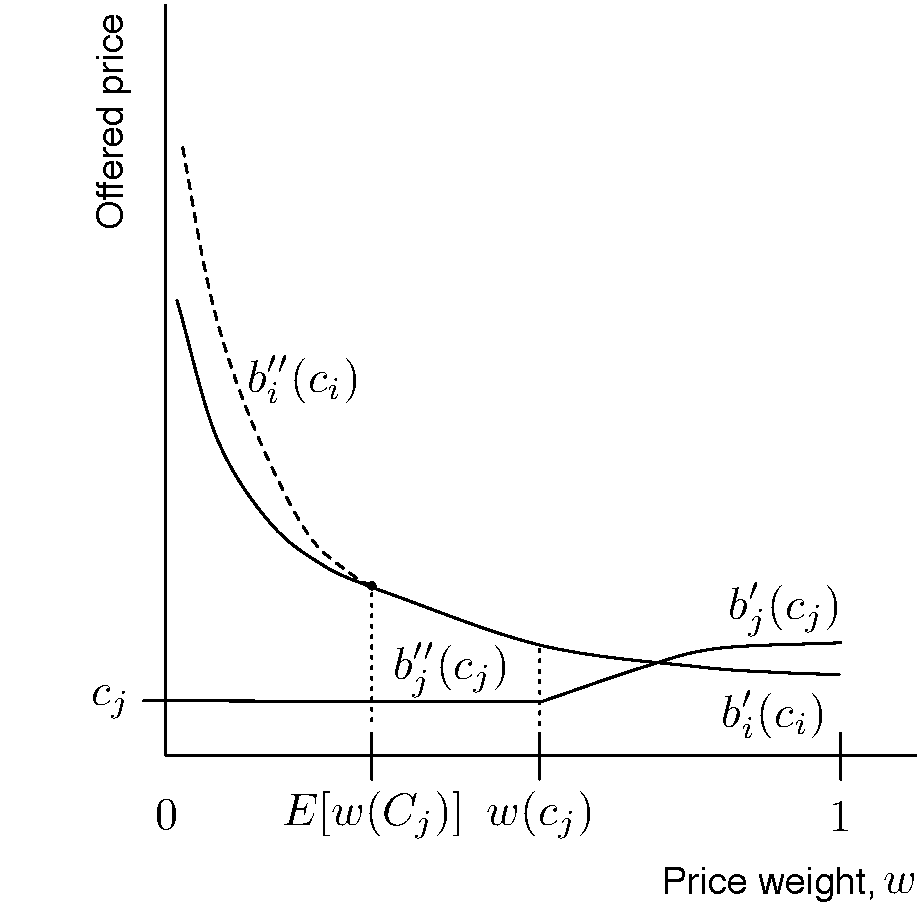
\includegraphics[width=3.5in]{2/Figures/pincomplete_bids_update_i_1}
	\label{fig:pincomplete_bids_update_i_1}
	\caption{Update in bidding strategy for network operator $j$ when $w(c_j) > E[w(C_j)]$}
	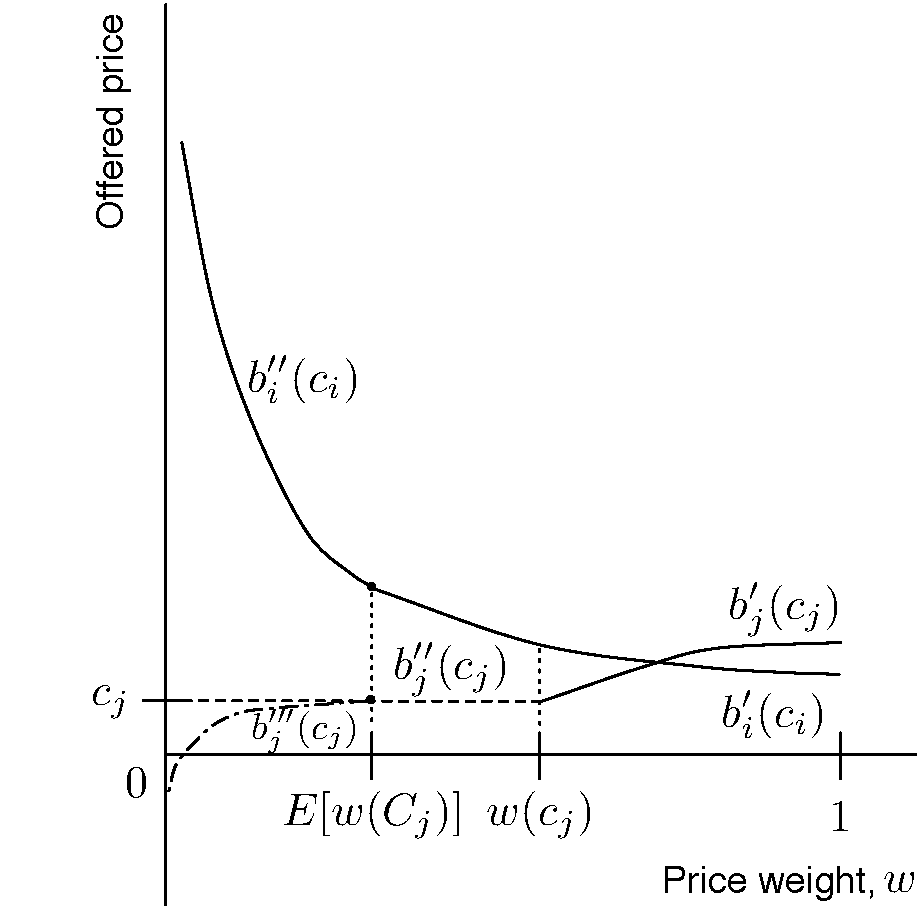
\includegraphics[width=3.5in]{2/Figures/pincomplete_bids_update_j_1}
	\label{fig:pincomplete_bids_update_j_1}
\end{figure}

\begin{figure}[tp!]
	\caption{Update in bidding strategy for network operator $i$ when $w(c_j) < E[w(C_j)]$}
	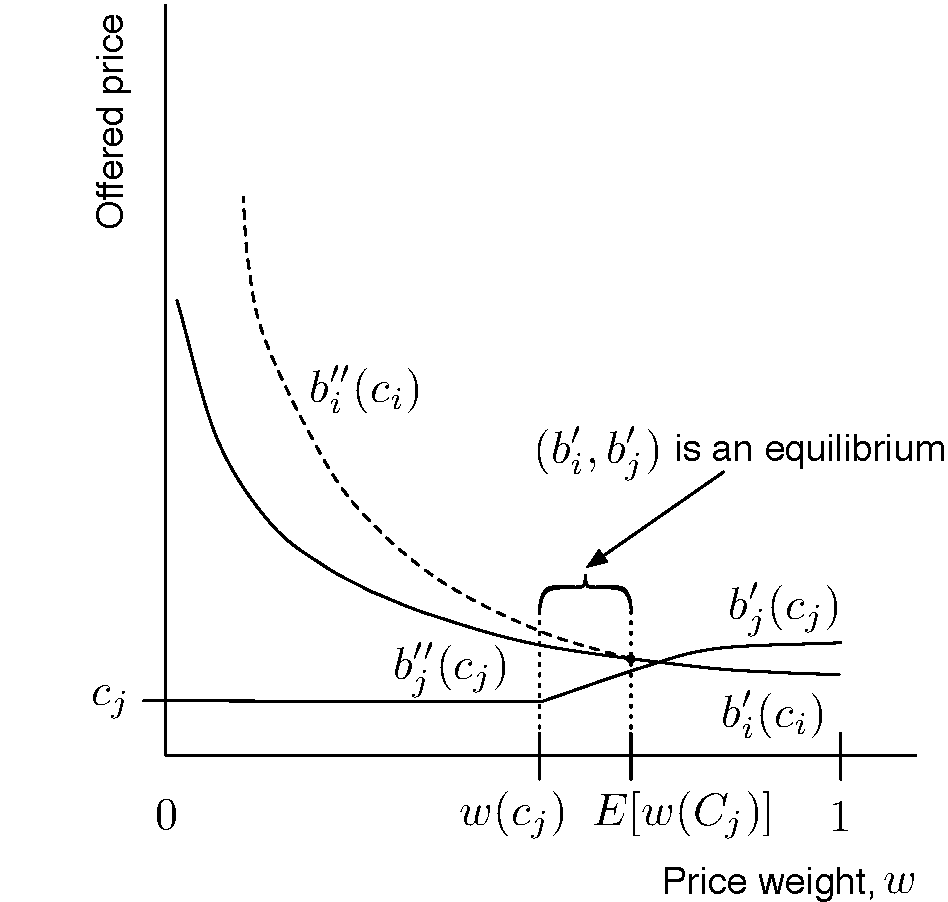
\includegraphics[width=3.5in]{2/Figures/pincomplete_bids_update_i_2}
	\label{fig:pincomplete_bids_update_i_2}
\end{figure}

Nevertheless, network operator $i$ might find it beneficial to update their bidding strategy given the fact that network operator $j$ bids according to $b_j''$ for $w<w(c_j)$, as this could potentially lead to higher profits for network operator $i$. However, there is at least one major limitation that network operator $i$ will face; that is, $w(c_j)$ as perceived by network operator $i$ is a function of cost of network operator $j$. Hence, it is a function of a random variable $C_j$. Since $C_j$ is a continuous random variable, the exact estimation of $w(C_j)$ is impossible; i.e., the probability of the event $w(C_j)=E[w(C_j)]$ is zero. Therefore, if network operator $i$ decides to update their bidding strategy, they may actually decrease their expected profits. To see why, suppose that network operator $i$ updates their bidding strategy. In this case, $b_j''(c_j) = c_j$ and $\lambda_i = 0$ which imply that $m_j = 0$, $n_j=1$ and thus
\begin{align*}
	&1 - b_i - \frac{1-w}{w}(r_i-r_j) - b_i + c_i = 0\\
	\iff &b_i''(c_i) = \frac{1}{2} - \frac{1-w}{2w}(r_i-r_j) + \frac{1}{2}c_i.
\end{align*}
If $w(c_j) > E[w(C_j)]$, then network operator $i$ will benefit from an update of their strategy; that is,
\begin{align*}
	&E\left[b_i''(c_i)-c_i \:\middle\vert\: wb_i''(c_i) + (1-w)r_i < wC_j + (1-w)r_j \right]\\
	- &E\left[b_i'(c_i)-c_i \:\middle\vert\: wb_i'(c_i) + (1-w)r_i < wC_j + (1-w)r_j \right] > 0
\end{align*}
for all $c_i\in[0,1]$ and $w < E[w(C_j)]$. Figure~\ref{fig:pincomplete_bids_update_i_1} depicts the above situation. Network operator $i$ will increase their bid (or offered price) for $w < E[w(C_j)]$, and yet will not decrease their probability of winning. At the same time, network operator $j$ will not have an incentive to modify their bidding strategy as it does not yield higher profits than by bidding $b_j''(c_j)$; that is, network operator $j$ faces an optimization problem
\begin{equation*}
	\max_{b_j} E\left[b_j - c_j \:\middle\vert\: wb_j + (1-w)r_j < wb_i''(C_i) + (1-w)r_i \right],
\end{equation*}
which yields
\begin{equation*}
	b_j'''(c_j) = \frac{1}{2}c_j - \frac{1-w}{4w}(r_j-r_i).
\end{equation*}
The difference in expected profits resulting from using $b_j'''$ for $w < E[w(C_j)]$ rather than $b_j''$ is negative; i.e.,
\begin{align*}
	&E\left[b_j'''(c_j)-c_j \:\middle\vert\: wb_j'''(c_j) + (1-w)r_j < wb_i''(C_i) + (1-w)r_i \right]\\
	- &E\left[b_j''(c_j)-c_j \:\middle\vert\: wb_j''(c_j) + (1-w)r_j < wb_i''(C_i) + (1-w)r_i \right] \le 0
\end{align*}
for all $c_j\in[0,1]$. Figure~\ref{fig:pincomplete_bids_update_j_1} depicts the above situation. Network operator $j$ would decrease their bid (or offered price) for $w < E[w(C_j)]$, and would bid below their cost.

If $w(c_j) < E[w(C_j)]$, then network operator $i$ will decrease their expected profits for $w(c_j) < w < E[w(C_j)]$, as in this range, the pair of bidding strategies $(b_i',b_j')$ constitutes an equilibrium. Figure~\ref{fig:pincomplete_bids_update_i_2} shows the above situation. However, it is not clear whether the increase in expected profits when $w(c_j) > E[w(C_j)]$ for network operator $i$ is larger than the decrease in expected profits when $w(c_j) < E[w(C_j)]$, and hence, whether it is worth for network operator $i$ to guess the value of $w(c_j)$.

The above discussion suggests that a possible solution to the constrained optimization problem in Equation~\eqref{eq:pcomp_exp_utility_c} may assume the following form
\begin{equation*}
	b_i^*(c_i) = \max\left\{ c_i, b_i'(c_i) \right\}.
\end{equation*}
However, since a formal proof is not provided, the result is stated as a conjecture.
\begin{conjecture}
\label{conj:pcomp_max_equi_bidding_str}
Let there be $n=2$ network operators. Suppose $c_i$ is independently drawn from uniform distribution over the interval $[0,1]$ for all $i\in N$, and $r_i\in [0,1]$ for all $i\in N$ is common knowledge. If the optimization problem is subject to a constraint $b_i\ge c_i$, then the equilibrium bidding strategy for all $w\in (0,1]$ is given by
\begin{equation}
\label{eq:pcomp_equi_bidding_str_max}
	b_i^*(c_i) = \max\left\{ c_i, b_i'(c_i) \right\}.
\end{equation}
\end{conjecture}
Plot figures~1.6 and~1.7 with the conjectured equilibrium bidding strategy in Equation~(1.34). FIX:ME
% subsubsection incomplete_information_n_2 (end)
% subsection direct_restricted_case_n_2_ (end)
% section direct_approach (end)

\section{Indirect Approach} % (fold)
\label{sec:indirect_approach}
In this section, the bidding problem will be transformed from a bidding problem with symmetric type (or cost) distributions into a bidding problem with asymmetric type distributions. This type of bidding problems has already been researched by the economic community, both in a very specific setting (two bidders, specific type distributions) \cite{KaplanZamir2007,MaskinRiley2000}, and in a very general setting ($n$ bidders, arbitrary type distributions) \cite{Lebrun1999,Lebrun2006}, and hence there exist results that are applicable to the problem at hand.

In order to transform the problem, recall the utility function for each network operator $i$
\begin{equation*}
  u_i(b,c,r) = \left\{
	\begin{array}{l l}
		b_i-c_i & \;\text{if } wb_i + (1-w)r_i < \displaystyle\min_{j\neq i}[wb_j + (1-w)r_j],\\
		0 & \;\text{if } wb_i + (1-w)r_i > \displaystyle\min_{j\neq i}[wb_j + (1-w)r_j],
	\end{array}\right.
\end{equation*}
and let
\begin{equation}
  \label{eq:b_hat}
  \hat{b}_i = wb_i + (1-w)r_i \quad\text{for all } i\in N.
\end{equation}
(Note that the new bid is just an alias for the compound bid, and in fact, they are equivalent; $\beta(b_i,r_i)\equiv\hat{b}_i$.) Solving Equation~\eqref{eq:b_hat} for $b_i$ yields
\begin{equation}
  \label{eq:b_from_b_hat}
  b_i = \frac{\hat{b}_i - (1-w)r_i}{w}, \quad w\neq 0.
\end{equation}
Substituting Equation~\eqref{eq:b_from_b_hat} back into the utility function yields
\begin{equation*}
  u_i(\hat{b},c,r) = \left\{
	\begin{array}{l l}
		\displaystyle\frac{1}{w}\left[\hat{b}_i-(wc_i + (1-w)r_i)\right] & \;\text{if } \hat{b}_i < \displaystyle\min_{j\neq i}\hat{b}_j,\\[2ex]
		0 & \;\text{if } \hat{b}_i > \displaystyle\min_{j\neq i}\hat{b}_j.
	\end{array}\right.
\end{equation*}
If we further let
\begin{equation}
  \label{eq:cost_hat}
  \hat{c}_i = wc_i + (1-w)r_i \quad\text{for all } i\in N,
\end{equation}
the utility function simplifies to
\begin{equation}
  \label{eq:sellers_utility_hat}
  u_i(\hat{b},\hat{c}) = \left\{
	\begin{array}{l l}
		\displaystyle\frac{1}{w}\left(\hat{b}_i-\hat{c}_i\right) & \;\text{if } \hat{b}_i < \displaystyle\min_{j\neq i}\hat{b}_j,\\[2ex]
		0 & \;\text{if } \hat{b}_i > \displaystyle\min_{j\neq i}\hat{b}_j.
	\end{array}\right.
\end{equation}
In order to avoid ambiguity, we shall refer to $\hat{c}_i$ as costs-hat and $\hat{b}_i$ as bids-hat, while still referring to $c_i$ as costs and $b_i$ as bids. Note, moreover, that since both $w$ and $r_i$ are assumed to be given to the network operators (i.e., they cannot directly modify their values), the costs-hat and bids-hat are simply convex (and hence, linear) combinations involving costs and bids respectively (Equations~\eqref{eq:b_hat}~and~\eqref{eq:cost_hat}). Therefore, a network operator bidding their cost-hat is equivalent to bidding their cost.

As a result of this transformation, the costs-hat, $\hat{c}_i$, for each network operator $i$ are distributed over the interval
\begin{equation*}
  \hat{c}_i\in [(1-w)r_i, (1-w)r_i + w]
\end{equation*}
since $c_i\in [0,1]$ for all $i\in N$. Note, moreover, that for all $i\in N$
\begin{equation*}
  [(1-w)r_i, (1-w)r_i + w] \subset [0,1]
\end{equation*}
since $w\in (0,1)$ and $r_i\in [0,1]$, and in particular, if $w=1$
\begin{equation*}
  [(1-w)r_i, (1-w)r_i + w] = [0,1].
\end{equation*}

With these results at hand, we can proceed with the analysis of the game.

\subsection{Generic Case} % (fold)
\label{sub:indirect_generic_case}
In the generic case, with arbitrary probability distributions of costs and $n\ge 2$ network operators, recall that: if $w=0$, then Proposition~\ref{prop:special_case_w_0} holds; if $w=1$, then Proposition~\ref{prop:special_case_w_1} holds; and if $r_i=r_j$ for all $i,j\in N$ such that $i\neq j$, then Corollary~\ref{cor:special_case_r_i_r_j_} holds. Therefore, it is sufficient to consider only the case when $w\in(0,1)$, and at least one network operator is characterized by a different reputation rating from the other network operators; that is, there exists $i\in N$ such that $r_i\neq r_j$ for all $i\neq j$ and $j\in N$.

Firstly, note that under the generic assumptions specified in Section~\ref{sec:problem_definition_and_assumptions}, the problem satisfies the following regularity conditions.
\begin{proposition}[Regularity Conditions]
\label{prop:regularity_conditions}
Let $F_i$ be the distribution function of $\hat{c}_i$ for all $i\in N$. Then,
\begin{enumerate}
  \item the support of $F_i$ is an interval ${[(1-w)r_i, (1-w)r_i + w]}$;
  \item $F_i$ is differentiable over ${((1-w)r_i, (1-w)r_i + w]}$ with a derivative $f_i$ locally bounded away from zero over this interval; and
  \item $F_i$ is atomless.
\end{enumerate}
\end{proposition}

The regularity conditions in Proposition~\ref{prop:regularity_conditions} correspond to the regularity assumptions on type distributions put forward by Lebrun~\cite{Lebrun2006} (cf. Assumptions~A.1 in~\cite{Lebrun2006}). Therefore, since our problem satisfies Lebrun's assumptions, his results are applicable to our problem, and we conclude that:
\begin{proposition}[Characterization of the Equilibrium]
\label{prop:characterisation_of_the_equilibrium}
$\quad$\\
\begin{enumerate}
  \item There exists a pure-strategy Bayesian Nash equilibrium where network operators submit at least their costs, and
  \item the pure-strategy Bayesian Nash equilibrium where network operators submit at least their costs is unique.
\end{enumerate}
\end{proposition}

However, even though the equilibrium exists and is unique, the establishment of a closed-form solution in a generic setting ($n\ge 2$ network operators and arbitrary cost distribution) is very difficult (if even possible) \cite{Lebrun2006, Krishna10}.
% subsection indirect_generic_case (end)

\subsection{Restricted Case $n=2$} % (fold)
\label{sub:indirect_restricted_case_n_2_}
It is possible to explicitly derive the equilibrium bidding strategy functions in a much restricted setting. Let $n=2$ network operators, and assume costs, $c_i$, for both network operators are drawn from the uniform distribution. The utility function becomes
\begin{equation*}
  u_i(\hat{b},\hat{c}) = \left\{
	\begin{array}{l l}
		\displaystyle\frac{1}{w}\left(\hat{b}_i-\hat{c}_i\right) & \;\text{if } \hat{b}_i < \hat{b}_j,\\[2ex]
		\displaystyle\frac{1}{2w}\left(\hat{b}_i-\hat{c}_i\right) & \;\text{if } \hat{b}_i = \hat{b}_j,\\[2ex]
		0 & \;\text{if } \hat{b}_i > \hat{b}_j.
	\end{array}\right.
\end{equation*}
Without loss of generality, suppose $r_i < r_j$. Since the distribution of costs, $c_i$, for each network operator $i$ is uniform with the support $[0,1]$, Equation~\eqref{eq:cost_hat} implies that the distribution of costs-hat, $\hat{c}_i$, for each network operator $i$ is uniform with the support~${[\underline{\hat{c}}_i, \bar{\hat{c}}_i]} = {[(1-w)r_i, (1-w)r_i + w]}$. Therefore, the distribution function of costs-hat satisfies the regularity conditions specified in Proposition~\ref{prop:regularity_conditions}, and by Proposition~\ref{prop:characterisation_of_the_equilibrium}, we conclude that the pure-strategy Bayesian Nash equilibrium where network operators submit at least their costs exists and is unique.

The derivation of the equilibrium involves three stages: 1) deriving equilibrium inverse bidding strategy functions using the procedure described by Kaplan and Zamir~\cite{KaplanZamir2007}; 2) numerically estimating the equilibrium bidding strategy functions by inverting the inverses; and 3) transforming the problem back to the original domain (from costs-hat and bids-hat back to costs and bids). Since $r_i < r_j$, this implies that $\bar{\hat{c}}_i < \bar{\hat{c}}_j$. It is, moreover, assumed that bids are bounded from above which implies that no network operator wins by bidding more than $\bar{\hat{c}}_j$ (since $\bar{\hat{c}}_i < \bar{\hat{c}}_j$). In particular, in equilibrium, there is no bid higher than $\bar{\hat{c}}_j$. Furthermore, it is assumed that, in equilibrium, a network operator with zero probability of winning bids their cost-hat. (This assumption guarantees both the existence and uniqueness of the equilibrium by Proposition~\ref{prop:characterisation_of_the_equilibrium}.)

If $\bar{\hat{c}}_i \le 2\underline{\hat{c}}_j - \bar{\hat{c}}_j$, then any pure-strategy Bayesian Nash equilibrium must have network operator $i$ always bidding $\underline{\hat{c}}_j$, and hence, always winning the auction at price $\underline{\hat{c}}_j$. This case shall be referred to as trivial. Therefore, in the non-trivial case, we must have $\bar{\hat{c}}_i > 2\underline{\hat{c}}_j - \bar{\hat{c}}_j$ (cf. Lemma~1 in Kaplan and Zamir~\cite{KaplanZamir2007}). In this range, an equilibrium consists of strictly increasing, differentiable bidding strategy functions $\hat{b}_i(\hat{c})$ and $\hat{b}_j(\hat{c})$. Let the inverses of these bidding strategy functions be denoted as $\hat{c}_i(\hat{b})$ with support $[\underline{\hat{b}}_i, \bar{\hat{b}}_i]$, and $\hat{c}_j(\hat{b})$ with support $[\underline{\hat{b}}_j, \bar{\hat{b}}_j]$. As Kaplan and Zamir~\cite{KaplanZamir2007} establish, these supports are identical, and equal to the common support $[\underline{\hat{b}}, \bar{\hat{b}}]$.

Suppose, therefore, that $\bar{\hat{c}}_i > 2\underline{\hat{c}}_j - \bar{\hat{c}}_j$ holds, and consider the optimization problem for network operator $i$
\begin{align*}
  &\max_{b} E \left[ b - \hat{c}_i \:\middle\vert\: b < \hat{b}_j \right]\\
  = &\max_{b} (b - \hat{c}_i)\cdot P\{b < \hat{b}_j\}\\
  = &\max_{b} (b - \hat{c}_i)\cdot P\{\hat{c}_j(b) < \hat{C}_j\}\\
  = &\max_{b} (b - \hat{c}_i)(1 - F_j(\hat{c}_j(b)),
\end{align*}
where $F_j$ is the distribution function of costs-hat for network operator $j$. The first-order condition yields
\begin{align}
  &1 - F_j(\hat{c}_j(b)) - (b - \hat{c}_i)f_j(\hat{c}_j(b))\cdot\frac{d}{db}\hat{c}_j(b) = 0 \nonumber \\
  \iff &1 - \frac{\hat{c}_j(b) - \underline{\hat{c}}_j}{\bar{\hat{c}}_j - \underline{\hat{c}}_j} = \frac{1}{\bar{\hat{c}}_j - \underline{\hat{c}}_j}(b - \hat{c}_i)\cdot\frac{d}{db}\hat{c}_j(b) \nonumber \\
  \iff &(\hat{c}_i(b) - b)\cdot\frac{d}{db}\hat{c}_j(b) = \hat{c}_j(b) - \bar{\hat{c}}_j,
  \label{eq:first_order_bidder_i}
\end{align}
where we have used the facts that $F_j$ is the distribution function of the uniform distribution with the support $[\underline{\hat{c}}_j, \bar{\hat{c}}_j]$, and at an equilibrium $\hat{c}_i = \hat{c}_i(b)$. Similarly, for network operator $j$ we have
\begin{equation}
  \label{eq:first_order_bidder_j}
  (\hat{c}_j(b) - b)\cdot\frac{d}{db}\hat{c}_i(b) = \hat{c}_i(b) - \bar{\hat{c}}_i.
\end{equation}

The following boundary conditions must hold in equilibrium (cf. boundary conditions in Kaplan and Zamir~\cite{KaplanZamir2007}):
\begin{enumerate}
  \item $\hat{c}_j(\bar{\hat{b}}) = \bar{\hat{b}}$, (the network operator bids their cost-hat when their probability of winning is zero),
  \item $\hat{c}_i(\bar{\hat{b}}) = \bar{\hat{c}}_i$, (the maximum cost-hat that gives network operator $i$ a positive probability of winning), and
  \item $\hat{c}_i(\underline{\hat{b}}) = \underline{\hat{c}}_i$ and $\hat{c}_j(\underline{\hat{b}}) = \underline{\hat{c}}_j$ (the lowest bid-hat of each network operator is reached for their lowest cost-hat).
\end{enumerate}
Integrating Equations~\eqref{eq:first_order_bidder_i}~and~\eqref{eq:first_order_bidder_j} bounded by the aforementioned boundary conditions results in the derivation of the equilibrium inverse bidding strategy functions. The derivation procedure is fully described in Kaplan and Zamir~\cite{KaplanZamir2007}; hence, we only provide the final result.
\begin{proposition}
\label{prop:inverse_equi_bidding_str}
Let there be $n=2$ network operators, and suppose $c_i$ is independently drawn from uniform distribution over the interval $[0,1]$ for all $i\in N$. Let for all $i\in N$
\begin{equation*}
  \hat{b}_i = wb_i + (1-w)r_i,\quad\text{and}\quad \hat{c}_i = wc_i + (1-w)r_i,
\end{equation*}
with
\begin{equation}
  \label{eq:cost_hat_bounds}
  \underline{\hat{c}}_i = (1-w)r_i,\quad \bar{\hat{c}}_i = (1-w)r_i + w.
\end{equation}
Then the equilibrium inverse bidding strategy functions for all $i\in N$ and $w\in (0,1)$ are given by
\begin{align}
  \label{eq:inverse_equi_bidding_str_i}
  \hat{c}_i(b) &= \bar{\hat{c}}_i + \frac{(\bar{\hat{c}}_j - \bar{\hat{c}}_i)^2}{(\bar{\hat{c}}_j + \bar{\hat{c}}_i - 2b)d_i \exp{\left(\displaystyle\frac{\bar{\hat{c}}_j - \bar{\hat{c}}_i}{\bar{\hat{c}}_j + \bar{\hat{c}}_i - 2b}\right)} + 4(\bar{\hat{c}}_j - b)},\\[2ex]
  \label{eq:inverse_equi_bidding_str_j}
  \hat{c}_j(b) &= \bar{\hat{c}}_j + \frac{(\bar{\hat{c}}_i - \bar{\hat{c}}_j)^2}{(\bar{\hat{c}}_i + \bar{\hat{c}}_j - 2b)d_j \exp{\left(\displaystyle\frac{\bar{\hat{c}}_i - \bar{\hat{c}}_j}{\bar{\hat{c}}_i + \bar{\hat{c}}_j - 2b}\right)} + 4(\bar{\hat{c}}_i - b)},
\end{align}
where
\begin{align}
  \label{eq:constant_d_i}
  d_i = \frac{\displaystyle\frac{(\bar{\hat{c}}_j - \bar{\hat{c}}_i)^2}{\underline{\hat{c}}_i - \bar{\hat{c}}_i} + 4(\underline{\hat{b}} - \bar{\hat{c}}_j)}{-2(\underline{\hat{b}} - \bar{\hat{b}})} \exp{\left(\displaystyle\frac{\bar{\hat{c}}_j - \bar{\hat{c}}_i}{2(\underline{\hat{b}} - \bar{\hat{b}})}\right)}, \\[2ex]
  \label{eq:constant_d_j}
  d_j = \frac{\displaystyle\frac{(\bar{\hat{c}}_i - \bar{\hat{c}}_j)^2}{\underline{\hat{c}}_j - \bar{\hat{c}}_j} + 4(\underline{\hat{b}} - \bar{\hat{c}}_i)}{-2(\underline{\hat{b}} - \bar{\hat{b}})} \exp{\left(\frac{\bar{\hat{c}}_i - \bar{\hat{c}}_j}{2(\underline{\hat{b}} - \bar{\hat{b}})}\right)},
\end{align}
and
\begin{equation}
  \label{eq:bid_bounds}
  \underline{\hat{b}} = \frac{\underline{\hat{c}}_i\underline{\hat{c}}_j - \displaystyle\frac{(\bar{\hat{c}}_i + \bar{\hat{c}}_j)^2}{4}}{\underline{\hat{c}}_i - \bar{\hat{c}}_i + \underline{\hat{c}}_j - \bar{\hat{c}}_j},\quad
  \bar{\hat{b}} = \frac{\bar{\hat{c}}_i + \bar{\hat{c}}_j}{2}.
\end{equation}
\end{proposition}
Note that the equilibrium inverse bidding strategy functions are inconvenient to work with: for a particular bid-hat value, they map into a particular cost-hat for either network operator. It would be more intuitive to work with their inverses, where for a particular cost-hat, we would get a particular bid-hat. Since it is difficult (if even possible) to analytically invert the equilibrium inverse bidding strategy functions in Equations~\eqref{eq:inverse_equi_bidding_str_i}~and~\eqref{eq:inverse_equi_bidding_str_j}, we resort to numerical methods for estimating the inverses for a particular set of cost-reputation pairs with respect to the price weights for both network operators. Without loss of generality, assume that $r_i < r_j$. The numerical procedure is then as follows.
\begin{enumerate}
  \item For a particular price weight $w$ and reputation ratings $r_i$ and $r_j$, calculate the costs-hat supports for both network operators; that is, the endpoints of the interval $[\underline{\hat{c}}_i, \bar{\hat{c}}_i]$ for network operator $i$, and $[\underline{\hat{c}}_j, \bar{\hat{c}}_j]$ for network operator $j$ (Equation~\eqref{eq:cost_hat_bounds}).
  \item If $\bar{\hat{c}}_i \le 2\underline{\hat{c}}_j - \bar{\hat{c}}_j$, then the equilibrium is trivial. Network operator $i$ bids the lower endpoint of the cost-hat support of network operator $j$; that is, network operator $i$ bids $\underline{\hat{c}}_j$ for all $\hat{c}\in [\underline{\hat{c}}_i, \bar{\hat{c}}_i]$. Network operator $j$, on the other hand, bids their cost-hat; that is, network operator $j$ bids $\hat{c}$ for all $\hat{c}\in [\underline{\hat{c}}_j, \bar{\hat{c}}_j]$.
  \item If $\bar{\hat{c}}_i > 2\underline{\hat{c}}_j - \bar{\hat{c}}_j$, then the equilibrium is nontrivial. Hence,
  \begin{enumerate}
    \item Calculate the common bids-hat support $[\underline{\hat{b}}, \bar{\hat{b}}]$ (Equation~\eqref{eq:bid_bounds}).
    \item For all $\hat{b}\in [\underline{\hat{b}}, \bar{\hat{b}}]$, calculate the corresponding costs-hat for both network operators using Equations~\eqref{eq:inverse_equi_bidding_str_i}~and~\eqref{eq:inverse_equi_bidding_str_j}.
    \item Since by assumption $r_i < r_j$, it follows that $\bar{\hat{c}}_i \le \bar{\hat{c}}_j$, and hence, $\bar{\hat{b}}\le \bar{\hat{c}}_j$. Thus, network operator $j$ bids their cost-hat, $\hat{c}_j(\hat{b}) = \hat{c}_j$  for all $\hat{b}\in [\bar{\hat{b}}, \bar{\hat{c}}_j]$.
  \end{enumerate}
\end{enumerate}

\begin{figure}[tp!]
	\caption{Compound bid plotted against the price weight}
	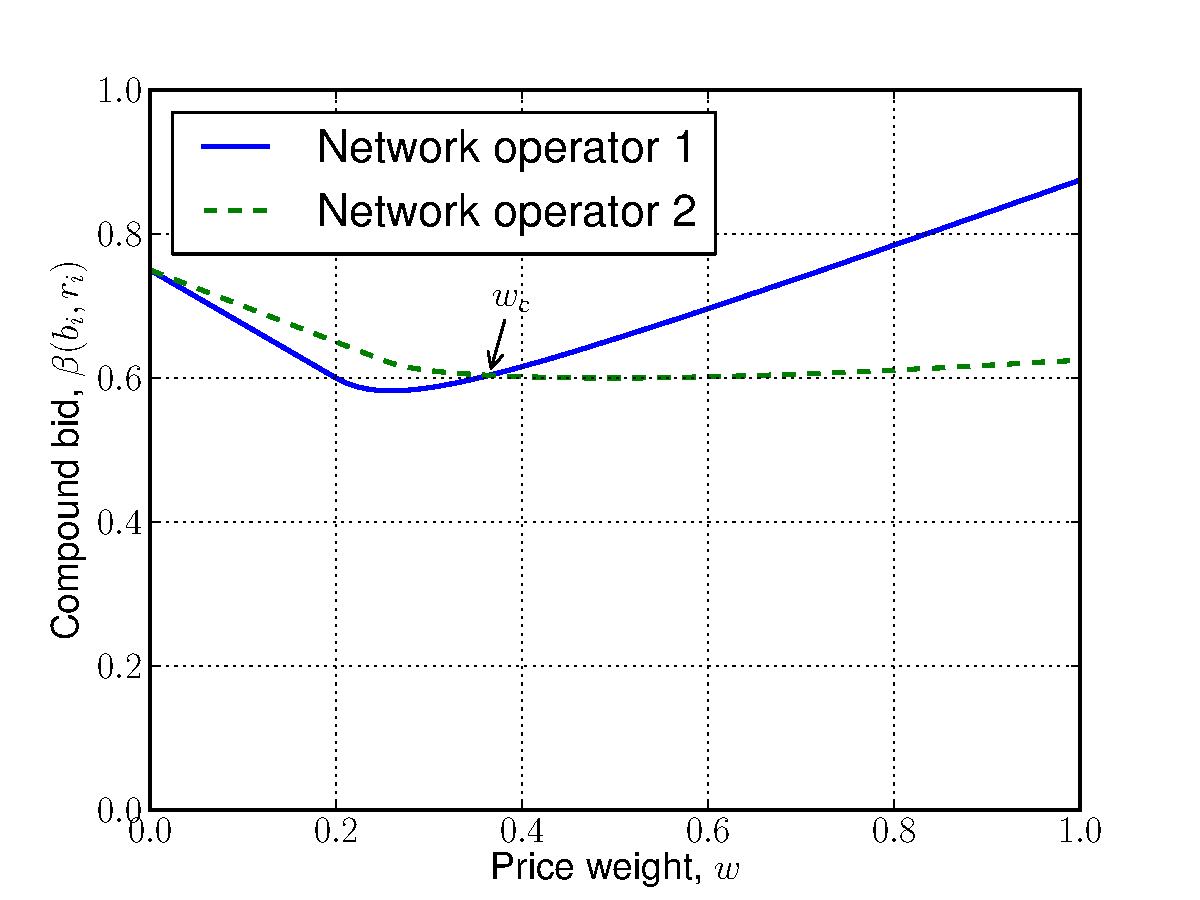
\includegraphics[width=\figsize]{2/Figures/indirect_bids}
	\label{fig:indirect_bids}
	\caption{Offered prices (bids) plotted against the price weight}
	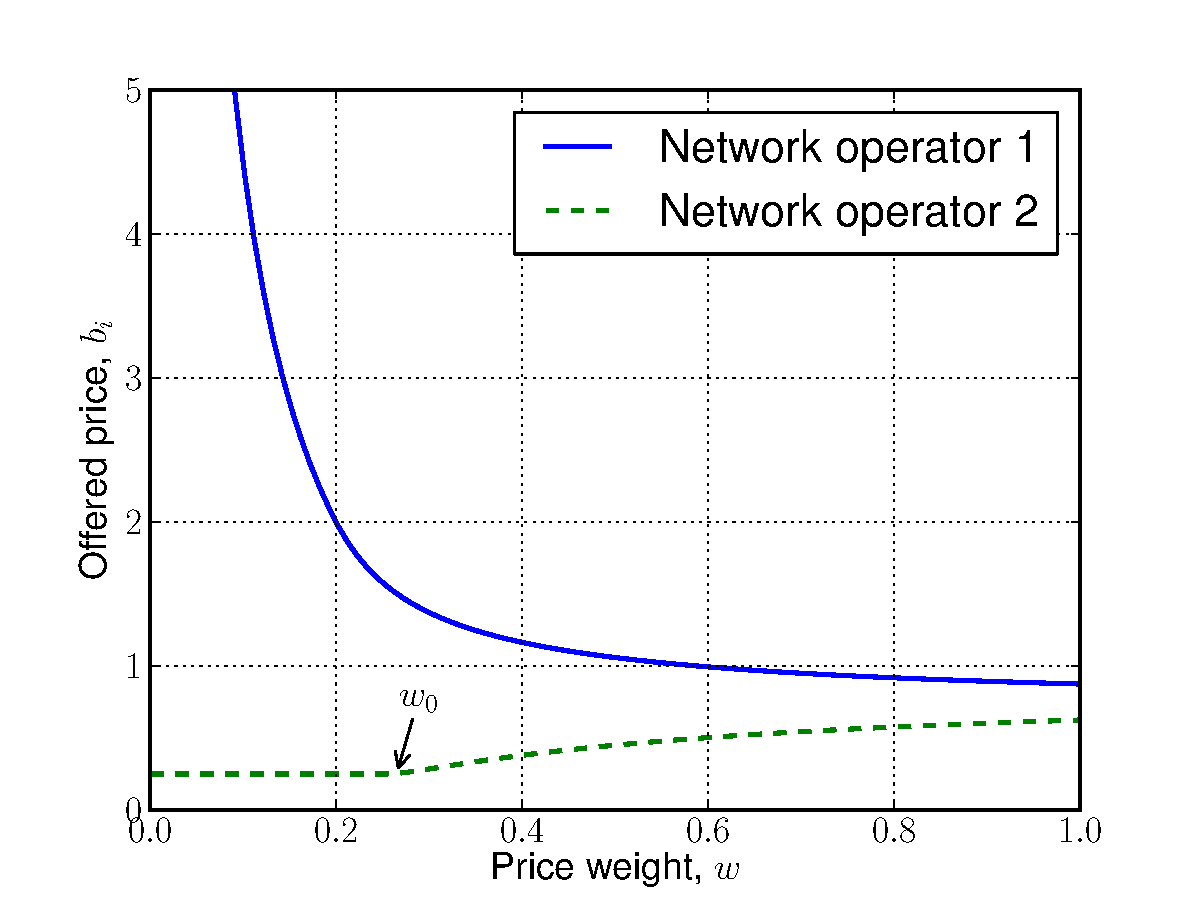
\includegraphics[width=\figsize]{2/Figures/indirect_prices}
	\label{fig:indirect_prices}
\end{figure}

The result of the steps described above is the tabulation of the costs-hat and their corresponding equilibrium bids-hat for a particular price weight $w$, and reputation ratings $r_i$ and $r_j$ for both network operators, in the ranges $[\underline{\hat{c}}_i, \bar{\hat{c}}_i]$ for network operator $i$ and $[\underline{\hat{c}}_j, \bar{\hat{c}}_j]$ for network operator $j$. Denote by
\begin{equation}
  \label{eq:equi_bidding_str_i}
  \hat{b}_i(\hat{c}_i) = \hat{b}_i \quad\text{for all } \hat{c}_i\in[\underline{\hat{c}}_i, \bar{\hat{c}}_i],
\end{equation}
and
\begin{equation}
  \label{eq:equi_bidding_str_j}
  \hat{b}_j(\hat{c}_j) = \hat{b}_j \quad\text{for all } \hat{c}_j\in[\underline{\hat{c}}_j, \bar{\hat{c}}_j]
\end{equation}
the resultant equilibrium bidding strategy functions.

The problem can be transformed back into the original domain by substituting Equations~\eqref{eq:b_hat}~and~\eqref{eq:cost_hat} into Equations~\eqref{eq:equi_bidding_str_i}~and~\eqref{eq:equi_bidding_str_j}; that is,
\begin{equation*}
  \hat{b}_i(\hat{c}_i) = \hat{b}_i \iff b_i = \displaystyle\frac{\hat{b}_i(wc_i + (1-w)r_i) - (1-w)r_i}{w}
\end{equation*}
for all $c_i\in[0,1]$, and
\begin{equation*}
  \hat{b}_j(\hat{c}_j) = \hat{b}_j \iff b_j = \displaystyle\frac{\hat{b}_j(wc_j + (1-w)r_j) - (1-w)r_j}{w}
\end{equation*}
for all $c_j\in[0,1]$.
Keeping costs and reputation ratings fixed, one can then estimate the equilibrium bidding strategy functions with respect to the price weights by sliding the value of $w\in(0,1)$.

By way of example, the equilibrium bidding strategy functions were estimated for the set of cost-reputation pairs depicted in Table~\ref{tab:pcomp}. Figure~\ref{fig:indirect_bids} shows the value of the compound bid, $\beta(b_i,r_i)$, for different values of $w$ for both network operators, while Figure~\ref{fig:indirect_prices} depicts the value of the monetary bid (or offered price), $b_i$, for different values of $w$ for both network operators. The numerical data in Table~\ref{tab:pcomp} suggests that network operator 2 should be the winner for the values of $w\rightarrow 1$ since network operator 2's cost is strictly lower than that of their opponent's. On the other hand, network operator 1 should be winner for the values of $w\rightarrow 0$ since network operator 1's reputation rating is strictly lower than that of their opponent's (which implies that network operator 1's reputation is in fact strictly higher than that of their opponent's). This prediction agrees with the numerical output shown in Figure~\ref{fig:indirect_bids}. Let $w_c$ denote the value of $w$ for which an intersection between the compound bids of both network operators occurs (if it exists). In Figure~\ref{fig:indirect_bids}, $w_c\approx 0.365$. Hence, network operator 2 wins the auction for the values of $w_c < w < 1$, while network operator 1 for the values of $0 < w < w_c$.

Note, furthermore, that since we have explicitly required the network operators to bid their own costs when their probability of winning is zero, the monetary bid of network operator 2 is capped at their cost, $b_2 = 0.25$, for the values of $0 < w \le w_0$ where $w_0\approx 0.265$ (Figure~\ref{fig:indirect_prices}). In the same range of $w$, as $w$ decreases, network operator 1's bid increases in an exponential-like fashion, to finally culminate in $b_1\to\infty$ at $w=0$ in accordance with Proposition~\ref{prop:special_case_w_0}. As $w\to 1$, on the other hand, the monetary bids of both network operators tend to the values specified in Proposition~\ref{prop:special_case_w_1}, that is, $b_1=0.875$ and $b_2=0.625$, to finally attain those values at $w=1$.
% subsection indirect_restricted_case_n_2_ (end)
% section indirect_approach (end)

\section{Discussion} % (fold)
\label{sec:discussion}
The aim of this section is twofold. First, the results from direct and indirect approaches are compared. Second, the prices the subscriber has to pay for each value of the price weight given a tuple of network operators' reputation ratings (in the restricted case) are examined.

\subsection{Comparison of Results from Direct and Indirect Approaches} % (fold)
\label{sub:comparison_of_results_from_direct_and_indirect_approaches}
If the network operators are assumed to submit at least their costs, then, in the restricted case, Proposition~\ref{prop:pcomp_equi_bidding_str} and Conjecture~\ref{conj:pcomp_max_equi_bidding_str} are ruled out by Proposition~\ref{prop:characterisation_of_the_equilibrium} combined with Proposition~\ref{prop:inverse_equi_bidding_str} since the latter establishes an analytical solution to the bidding problem while Proposition~\ref{prop:characterisation_of_the_equilibrium} makes this solution unique. Furthermore, for the same reason, Proposition~\ref{prop:characterisation_of_the_equilibrium} and Proposition~\ref{prop:inverse_equi_bidding_str} prove Conjecture~\ref{conj:special_case_w_1} for $n=2$ network operators and costs drawn from uniform distribution over the interval $[0,1]$ (cf. numerical example in Section~\ref{sub:indirect_restricted_case_n_2_}).

However, if this assumption is relaxed, then, as showed by Kaplan and Zamir~\cite{KaplanZamir2011}, Proposition~\ref{prop:characterisation_of_the_equilibrium} need no longer hold, and hence, there may exist multiple equilibria in the first-price sealed-bid auction bidding problem. As a result, both equilibria summarized in Proposition~\ref{prop:inverse_equi_bidding_str} as well as Proposition~\ref{prop:pcomp_equi_bidding_str} are valid. Kaplan and Zamir~\cite{KaplanZamir2011}, who characterize equilibria like the one specified in Proposition~\ref{prop:pcomp_equi_bidding_str} as non-standard, further argue that such equilibria are important and should not be neglected.
% subsection comparison_of_results_from_direct_and_indirect_approaches (end)

\begin{figure}[tp!]
  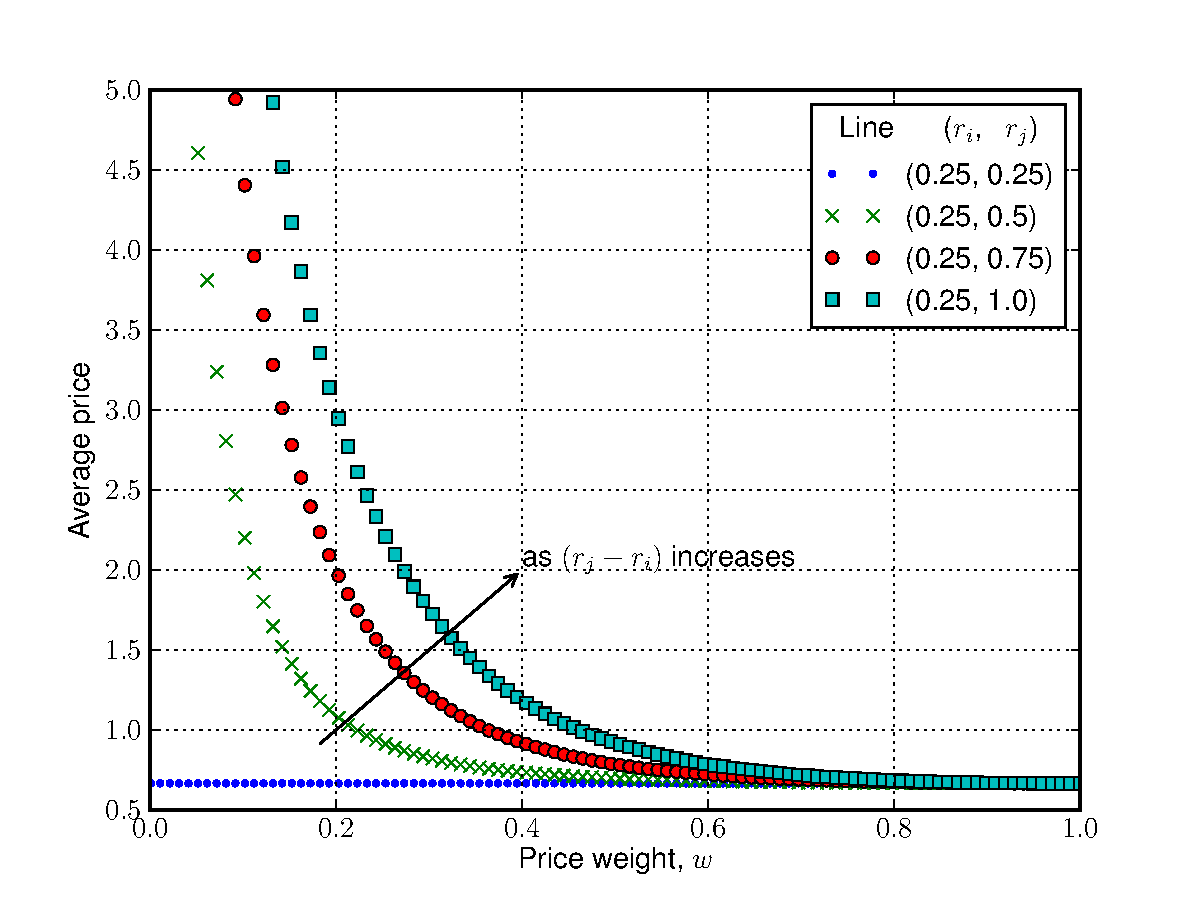
\includegraphics[width=\figsize]{2/Figures/expected_prices}
  \caption{Average prices plotted against the price weight for different pairs of reputation ratings}
  \label{fig:expected_prices}
  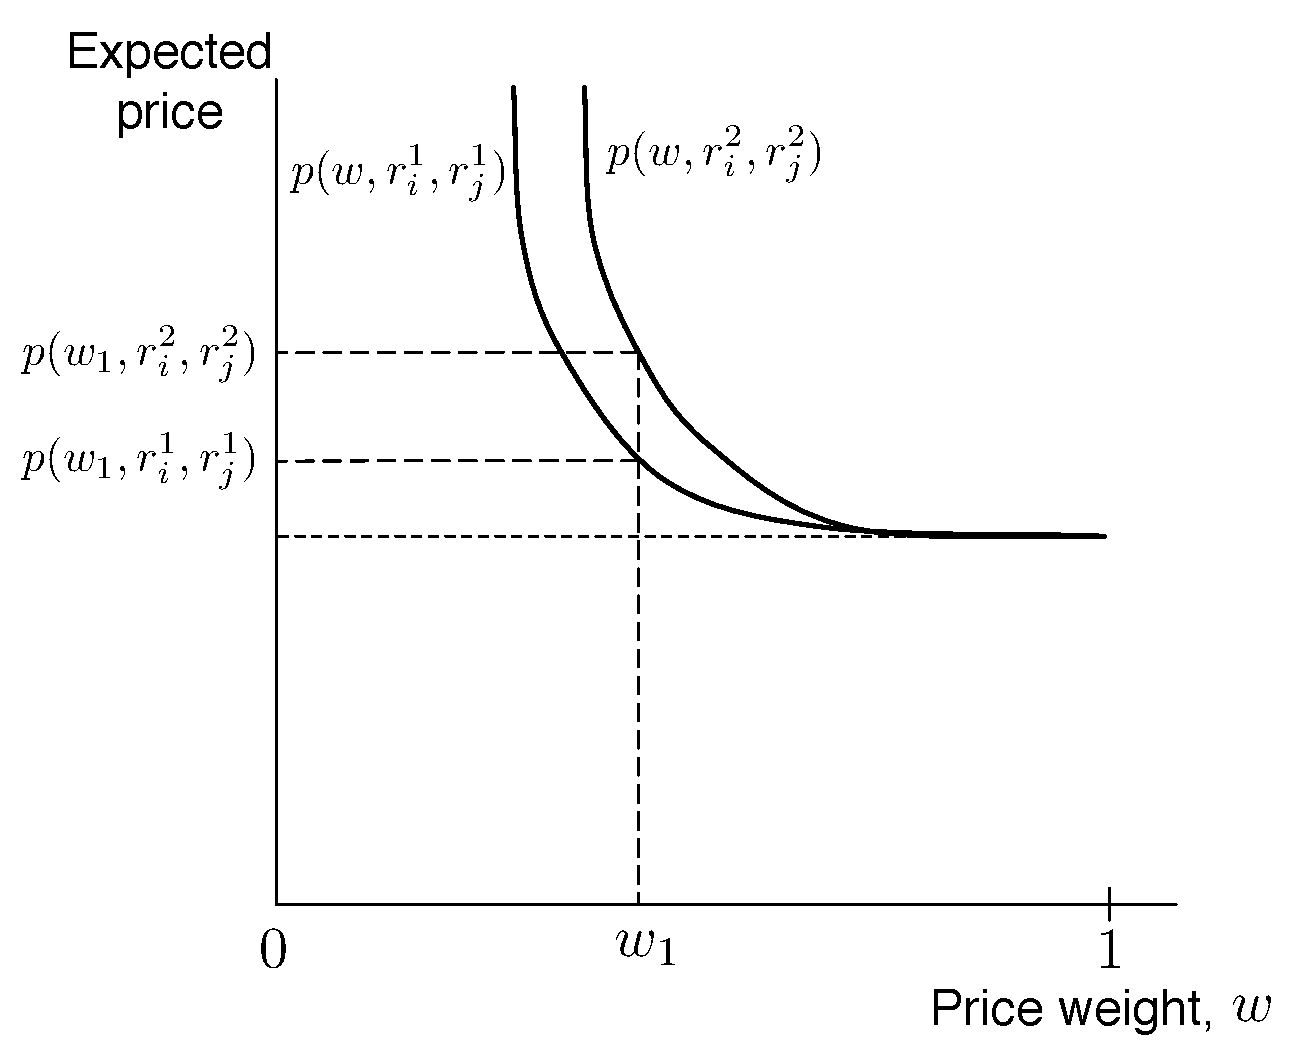
\includegraphics[width=\figsize]{2/Figures/expected_prices_sensitivity}
  \caption{Sensitivity of the price weight to the expected prices}
  \label{fig:expected_prices_sensitivity}
\end{figure}

\subsection{Subscriber's Perspective: Expected Prices in Restricted Case} % (fold)
\label{sub:subscriber_s_perspective_expected_prices_in_restricted_case}
Having derived the equilibrium bidding strategy functions in the restricted case, it is possible to examine the expected prices the subscriber will have to pay for different values of the price weight given the reputation ratings of the network operators. We consider only the equilibrium bidding strategy functions in Proposition~\ref{prop:inverse_equi_bidding_str} since they assume the network operators submit at least their costs. Hence, suppose all of the assumptions of Section~\ref{sub:indirect_restricted_case_n_2_} hold; that is, there are two network operators, and costs are uniformly distributed over the interval $[0,1]$. The expected price is equivalent to the expected value of the winning bid; that is, with some abuse of notation
\begin{equation}
  \label{eq:exp_price_def}
  E[p](w,r_i,r_j) = E[b_i \:\vert\: \arg\min_{i\in N}\beta(w,b_i,r_i)],
\end{equation}
where $b_i$ is the equilibrium bid, and $\beta(w,b_i,r_i) = \beta(b_i,r_i)$ evaluated for a particular value of $w$ for all $i\in N$.

If both network operators have equal reputation ratings, $r = r_i = r_j$ say, then Corollary~\ref{cor:special_case_r_i_r_j_} holds for all $w\in [0,1]$. Therefore, regardless of the choice of the price weight, the subscriber expects to pay the price of
\begin{equation}
  \label{eq:exp_price_at_w_1}
  E[p^*] \equiv E[p](w,r,r) = E\left[\min_{i\in N}\frac{1+c_i}{2}\right] \quad\text{for all } w\in [0,1],
\end{equation}
which is equivalent to Equation~\eqref{eq:standard_fpa} evaluated at $n=2$. In particular, for costs, $c_i$, uniformly distributed over the interval $[0,1]$, $E[p^*] = \frac{2}{3}$.

If, on the other hand, both network operators are characterized by different reputation ratings, then an analytical derivation of the expected prices for each value of the price weight given a pair of reputation ratings is cumbersome. This is due to the fact that network operators bid according to a pair of inverse equilibrium bidding functions specified in Proposition~\ref{prop:inverse_equi_bidding_str}, which are not easily invertible. Hence, we resort to numerical methods for estimating average (sample mean) prices for selected values of the price weight given a pair of reputation ratings.

To this end, for any given pair of reputation ratings, the costs are pseudo-randomly drawn from the uniform distribution over the discretized interval $[0,1]$. For each selected price weight, the average price is averaged over 10,000 i.i.d.~observations. The Strong Law of Large Numbers (which is stated in Section~\ref{sub:notation_probability}) implies that as the number of observations tends to infinity, the average (sample mean) of the observations approaches the real mean of the distribution of the random variable in question. Therefore, an average of 10,000 observations of the price for each selected price weight should provide a reasonable approximation of the expected price for that price weight. Without loss of generality, suppose further that $r_i \le r_j$. Figure~\ref{fig:expected_prices} shows the result of the estimation for four pairs of reputation ratings: $(r_i, r_j) = (0.25, 0.25)$, $(0.25, 0.5)$, $(0.25, 0.75)$, and $(0.25, 1.0)$.

It can be observed that regardless of the values of the reputation ratings, the expected prices, $E[p](w,r_i,r_j)$, are bounded from below by $E[p^*]$ for each price weight; this is depicted in Figure~\ref{fig:expected_prices}. Hence, it can be concluded that regardless of the values of the reputation ratings, the lowest expected price is achieved for $w=1$, and will not decrease as $w$ decreases; in fact, it can only either increase or remain constant.

Furthermore, as the difference $(r_j-r_i)$ increases, the expected prices, $E[p](w,r_i,r_j)$, increase as the price weight decreases; this is depicted in Figure~\ref{fig:expected_prices}. Therefore, it can be hypothesized that the smaller the difference $(r_j-r_i)$, the less (expected) price sensitive the price weight; that is, for any $w_1\in[0,1]$, if $(r^2_j-r^2_i) > (r^1_j-r^1_i)$ for all $r^1_i,r^1_j,r^2_i,r^2_j\in [0,1]$, then $E[p](w_1,r^2_i,r^2_j) \ge E[p](w_1,r^1_i,r^1_j)$ (Figure~\ref{fig:expected_prices_sensitivity}). In other words, for any expected price, as the difference $(r_j-r_i)$ between the reputation ratings of the network operators increases, the price weight has to increase (or remain constant) in order to keep the expected price fixed.
% subsection subscriber_s_perspective_expected_prices_in_restricted_case (end)
% section discussion (end)

\section{Summary} % (fold)
\label{sec:summary_ch2}

% section summary_ch2 (end)

\section{Proofs} % (fold)
\label{sec:proofs}
\begin{proof}[Proof of Proposition~\ref{prop:special_case_w_0}]
Let $m = |N_0|$ be the number of network operators with the lowest reputation rating such that $m\in\mathbb{Z}_+$. Since $n = |N|$ is finite and $N_0\subseteq N$, then $m \le n$. Now, each $j\in N_0$ is facing a maximization problem
\begin{equation*}
	\max_{b_j} \frac{1}{m} \left(b_j - c_j \right), \quad\text{for all } j\in N_0.
\end{equation*}
Since $1\le m\le n$, and since $b_j\in\mathbb{R}_+$ and $\mathbb{R}_+$ is not bounded from above, this implies that the maximization problem is unbounded; that is, $b_j\rightarrow\infty$ for all $j\in N_0$.

The remaining network operators $k\in N\setminus N_0$ will try to solve
\begin{equation*}
	\max_{b_k} 0, \quad\text{for all } k\in N\setminus N_0,
\end{equation*}
since $r_k > r_j = \min_{i\in N} r_i$. Hence, each network operator $k\in N\setminus N_0$ is indifferent to the value of their bid, which concludes the proof.
\end{proof}

\begin{proof}[Proof of Proposition~\ref{prop:special_case_w_1}]
The proof is analogous to the proof of Proposition~2.2 in Krishna~\cite{Krishna10}.
\end{proof}

\begin{proof}[Proof of Proposition~\ref{prop:pcomp_equi_bidding_str}]
Suppose there are two network operators: network operator 1 and 2 with cost-reputation pairs $(c_1,r_1)$ and $(c_2,r_2)$ respectively. Suppose that network operator 2 follows $b_2'$ equilibrium bidding strategy. We will argue that it is optimal for network operator 1 to follow $b_1'$ equilibrium bidding strategy. First, note that $b_1'$ is strictly increasing and continuous function of cost (similarly is $b_2'$). Suppose that network operator 1 bids an amount $b_1$. Since $b_1'$ is strictly increasing, it is bijective. Therefore, there exists unique cost $\hat{c}_1$ such that $\hat{c}_1 = {b_1'}^{-1}(b_1)$. Network operator 1's expected utility from bidding $b_1'(\hat{c}_1)$ is
\begin{align*}
	&\tilde{u}_1(b_1'(\hat{c}_1), c_1) \\
	&= E \left[ b_1'(\hat{c}_1) - c_1 \:\middle\vert\: wb_1'(\hat{c}_1) + (1-w)r_1 < wb_2'(c_2) + (1-w)r_2 \right] \\
	&= \frac{1}{2} \left( 1 - \frac{2}{3}\cdot\frac{1-w}{w}(r_1-r_2) + \hat{c}_1 - 2c_1 \right) \left( 1 - \hat{c}_1 - \frac{2}{3}\cdot\frac{1-w}{w}(r_1-r_2) \right).
\end{align*}
We thus obtain that
\begin{equation*}
	\tilde{u}_1(b_1'(c_1), c_1) - \tilde{u}_1(b_1'(\hat{c}_1), c_1) = \frac{1}{2}(c_1-\hat{c}_1)^2 \ge 0
\end{equation*}
regardless of whether $\hat{c}_1\ge c_1$ or $\hat{c}_1 \le c_1$. We have thus argued that if network operator 2 follows $b_2'$, network operator 1 with a cost $c_1$ cannot benefit by bidding anything other than $b_1'(c_1)$. Similar argument can be used to show that it is optimal for network operator 2 to follow $b_2'$ while network operator 1 is following $b_1'$. Hence, $(b_1',b_2')$ constitutes a Bayesian-Nash equilibrium profile.
\end{proof}

\begin{proof}[Proof of Proposition~\ref{prop:pcomp_negative_bids}]
Let there be two network operators: network operator 1 and 2 with cost-reputation pairs $(c_1,r_1)$ and $(c_2,r_2)$ respectively. Suppose that both network operators follow the equilibrium bidding strategy, $b_i'(c_i)$. We need to show that network operator 1's bid is always at least as high as their cost whenever they win or draw with network operator 2; that is, $b_1'(c_1)\ge c_1$.

First of all, note that if $r_1\le r_2$,
\begin{equation*}
	b_1'(c_1) = \frac{1}{2}-\frac{1-w}{3w}(r_1-r_2) + \frac{1}{2}c_1 \ge \frac{1}{2}(1+c_1) \ge c_1, \quad\text{for all } c_1\in[0,1].
\end{equation*}
Thus, we need only to consider the case when $r_1>r_2$.

Suppose $r_1>r_2$. If $c_1>c_2$, and since $b_1'(c_2)$ is strictly increasing in $c_1$, network operator 1 will lose for all values of $w\in(0,1]$. If $c_1=c_2$, network operator 1 will lose for all values of $w\in(0,1)$, except at $w=1$ when there will be a draw. But at $w=1$, network operator 1's bid is at least as high as her cost; i.e.,
\begin{equation*}
	b_1'(c_1) = \frac{1}{2}(1+c_1) \ge c_1, \quad\text{for all } c_1\in[0,1].
\end{equation*}
If $c_1<c_2$, it is sufficient to show that the intersection of $b_1'(c_1)$ and $c_1$ in terms of $w$ can never occur before the intersection of $\beta(b_1'(c_1),r_1)$ and $\beta(b_2'(c_2),r_2)$. First of all, we need to check that both intersections do occur; that is,
\begin{equation*}
	b_1'(c_1) = c_1 \iff w = \frac{1}{1 + \frac{3}{2}\cdot\frac{1 - c_1}{r_1 - r_2}}.
\end{equation*}
Similarly,
\begin{equation*}
	\beta(b_1'(c_1),r_1) = \beta(b_2'(c_2),r_2) \iff w = \frac{1}{1+ \frac{3}{2}\cdot\frac{c_2-c_1}{r_1-r_2}}.
\end{equation*}
Since $r_1>r_2$ and $c_1<c_2$, we have $0<r_1-r_2\le 1$ and $0<c_2-c_1\le 1$. Therefore, this implies
\begin{equation*}
	0 < w = \frac{1}{1+ \frac{3}{2}\cdot\frac{1-c_1}{r_1-r_2}} \le 1,
\end{equation*}
and
\begin{equation*}
	0 < w = \frac{1}{1+ \frac{3}{2}\cdot\frac{c_2-c_1}{r_1-r_2}} \le 1.
\end{equation*}
Now, suppose that the intersection of $b_1'(c_1)$ and $c_1$ occurs before that of $\beta(b_1'(c_1),r_1)$ and $\beta(b_2'(c_2),r_2)$. We must thus have
\begin{equation*}
	\frac{1}{1+\frac{3}{2}\cdot\frac{c_2-c_1}{r_1-r_2}} < \frac{1}{1+\frac{3}{2}\cdot\frac{1-c_1}{r_1-r_2}} \iff \frac{1-c_2}{r_1-r_2} < 0.
\end{equation*}
But since $c_2\in[0,1]$ and $r_1>r_2$ by assumption,
\begin{equation*}
	0 < \frac{1-c_2}{r_1-r_2}
\end{equation*}
we reach a contradiction, and this concludes the proof.
\end{proof}

\begin{proof}[Proof of Proposition~\ref{prop:pcomp_direct_mechanism}]
Let there be two network operators: network operator 1 and 2 with cost-reputation pairs $(c_1,r_1)$ and $(c_2,r_2)$ respectively. Suppose that both network operators participate in the direct mechanism $(\mathbf{Q},\mathbf{M})$. Firstly, we show that the mechanism is incentive compatible. Without loss of generality, suppose that network operator 2 truthfully submits their cost to the mechanism. We argue that it is optimal for network operator 1 to also submit their cost truthfully. Suppose to the contrary; that is, that network operator 1 has an incentive not to reveal their cost truthfully by submitting $\hat{c}_1$. Thus, their expected utility becomes
\begin{align*}
	&\tilde{\tilde{u}}_1(\hat{c}_1) = E\left[ b_1'(\hat{c}_1) - c_1 \:\middle\vert\: 2b_1'(\hat{c}_1) - 1 + \frac{4}{3}\cdot\frac{1-w}{w}(r_1-r_2) < C_2 \right] \\
	&= \left(\frac{1}{2} - \frac{1}{3}\cdot\frac{1-w}{w}(r_1-r_2) + \frac{1}{2}\hat{c}_1 - c_1 \right)\left(1 - \hat{c}_1 - \frac{2}{3}\cdot\frac{1-w}{w}(r_1-r_2)\right).
\end{align*}
The first-order condition yields $\hat{c}_1 = c_1$ and the second-order condition is satisfied. Hence, this shows that $(\mathbf{Q},\mathbf{M})$ is incentive compatible.

Secondly, we show that $(\mathbf{Q},\mathbf{M})$ is individually rational. Since the mechanism is incentive compatible, each network operator reveals their cost truthfully. Hence, for all $c_1$
\begin{align*}
	\tilde{\tilde{u}}_1(c_1) &= \left(\frac{1}{2} - \frac{1}{3}\cdot\frac{1-w}{w}(r_1-r_2) - \frac{1}{2}c_1 \right)\left(1 - c_1 - \frac{2}{3}\cdot\frac{1-w}{w}(r_1-r_2)\right)\\
	&= \frac{1}{2}\left( 1 - c_1 - \frac{2}{3}\cdot\frac{1-w}{w}(r_1-r_2) \right)^2 \ge 0.
\end{align*}
Therefore, $(\mathbf{Q},\mathbf{M})$ is individually rational.
\end{proof}

\begin{proof}[Proof of Proposition~\ref{prop:regularity_conditions}]
Proof of 1) is trivial. To prove 2) and 3), we note that for all $x\in [(1-w)r_i, (1-w)r_i + w]$,
\begin{align*}
  F_i(x)
  &= P\{\hat{C}_i\le x\} \\
  &= P\{wC + (1-w)r_i\le x\} \\
  &= P\left\{ C\le \frac{x - (1-w)r_i}{w} \right\}
\end{align*}
since $\hat{c}_i = wc_i + (1-w)r_i$ and $w\neq 0$. Hence,
\begin{equation*}
  F_i(x) = F_C\left( \frac{x - (1-w)r_i}{w} \right)
\end{equation*}
and
\begin{equation*}
  \frac{x - (1-w)r_i}{w}\in [0,1]
\end{equation*}
for all $x\in [(1-w)r_i, (1-w)r_i + w]$. Therefore, since $F_C$ is differentiable over $(0,1]$ with a derivative $f_C$ locally bounded away from zero over this interval, by extension, $F_i$ is differentiable over $((1-w)r_i, (1-w)r_i + w]$ with a derivative $f_i$ locally bounded away from zero over this interval, and this proves 2). Moreover, since $F_C$ is atomless, by extension, $F_i$ is atomless, and this proves 3).
\end{proof}

\begin{proof}[Proof of Proposition~\ref{prop:characterisation_of_the_equilibrium}]
Since both $w$ and $r_i$ are assumed to be given to the network operators (i.e., they cannot directly modify their values), the costs-hat and bids-hat are simply convex (and hence, linear) combinations involving costs and bids respectively (Equations~\eqref{eq:b_hat}~and~\eqref{eq:cost_hat}). Therefore, a network operator bidding their cost-hat is equivalent to bidding their cost. Hence, to prove 1) we note that Lebrun~\cite{Lebrun2006} proves the existence of a pure-strategy Bayesian Nash equilibrium where network operators submit at least their costs-hat (cf. C.5 Characterization with Possibly Different Lower and Upper Extremities in~\cite{Lebrun2006}). But since costs-hat are equivalent to costs, this also proves the existence of a pure-strategy Bayesian Nash equilibrium where network operators submit at least their costs.

To prove 2) we note that since $r_i\neq r_j$ for at least one network operator $i\in N$ such that $i\neq j$ and $j\in N$, then either $r_i < r_j$ or $r_i > r_j$. Without loss of generality, assume $r_i < r_j$ which implies that $(1-w)r_i < (1-w)r_j$ for all $w\in (0,1)$. By Theorem~1 in Lebrun~\cite{Lebrun2006}, the additional condition (ii) holds, and hence, the considered first-price auction has one and only one pure-strategy Bayesian Nash equilibrium where network operators bid at least their costs-hat. But since costs-hat are equivalent to costs, this also proves the uniqueness of a pure-strategy Bayesian Nash equilibrium where network operators submit at least their costs.
\end{proof}

\begin{proof}[Proof of Proposition~\ref{prop:inverse_equi_bidding_str}]
The proof is analogous to the proof of Proposition~1 in Kaplan and Zamir~\cite{KaplanZamir2007}.
\end{proof}
% section proofs (end)

% chapter selling_mechanism_in_the_digital_marketplace (end)
